% Question to answers during the next chapters
%%% Instruments used, set-up, materials
%%Description of the instruments and materials
%%How the instruments are set-up and what auxiliary connections might need to be used.
%%% add statment
\chapter{Algorithm to Optimize the Sailing Path for Laser Classes.} \label{sec:AlgOptSail}
%Introduction
The optimization problem for the minimal path is a problem frequently related with logistics and operations research. This type of problem is usually related with the \textit{Euclidean} shortest path and solved either with networking optimization or dynamic programming (\textit{\acrshort{dp}}). Although for Olympic sailing classes the optimal path is not related with distance but with time instead. \par \noindent 
Because of this, the research of this type of problem on sports is limited and it is mainly focused on yacht competitions. Whereas the laser class is the smallest and one of the most used sailboats on Olympic Classes. The objective of this section is not only to explain widely used methods but their elements and how they should apply to develop and algorithm for the Laser Olympic class.\par

Many techniques used on \acrshort{dp} and networking optimization can be used in combination with the \acrshort{vmg} criterion to developed and optimization algorithm for laser races.  Because the target's location and the geometrical domain are the features that allows the used of both criteria thus the optimal solution is found inside the polygon \cite{mitchell2000geometric}.\par 

The first part of this chapter explains how chapter \ref{ch:physics_sailboat} and chapter \ref{ch:weatherModel} are integrated to develop the algorithm to optimized the path of laser boats and obtain a minimal time path. But because most of the formulas on section \ref{sec:equil_equat} are generic, the adjustments required to describe the laser class are explained in the second part of this chapter. Followed by the explanation about the algorithm, details such as the objective function, the constraints and its validation. The validation of the algorithm is at the end of the chapter, and it provides information about the parameters defined by the user and at the initialization of the algorithm. \par 

%\section{Incorporation of the Wind Model into a Path Algorithm}
\section{Weather Routing Models and Path Algorithms for Sailboats}\label{sec:weatherRoute}

Uncertainty weather is a typical condition that not only yacht competitions have to manage but also maritime transportation. The direction-dependency of the vessel's velocity is seen as a series of regions where the flow's velocity is designed as uniform. This is characterizes as an anisotropic medium condition, and path algorithm problems with this characteristic has been solved with different methods \cite{dolinskaya2013fastest}. \par 
\noindent 
The most used methods related with vessels or yachts and anisotropic medium come from operations research and logistics. For example, from operations research these methods are dynamic programming (\acrshort{dp}), direct and indirect methods while the networking method is related with logistics. \cite{kelly2015transcription},\cite{mitchell2000geometric}. In the networking method the order in which the locations can be reach is not as important than time. \par 
The formulation of the problem is focus on the time and not in the length of the trajectory. However, it is the velocity of the sailboat the one that determines the direction of the sailboat and considers the wind properties. Because of this, equation \ref{eq:rabaudmintime} defines the time of the path to displace a sailboat between 2 points \cite{rabaudoptimal}. This is the easiest formulation of the problem but it shows how this problem differs from the shortest path approach.  \par

\begin{equation} \label{eq:rabaudmintime}
\begin{aligned}
T_{AB}=\int_{A}^{B} dt=\int_{A}^{B} \frac{dl}{v}  \\
\end{aligned}
\end{equation}

\subsection{Dynamic Programming and direction-dependence for Path Algorithms} \label{sec:dynProg}

\acrshort{dp} is a widely used technique to solve the optimal path problem for yachts and maritime transportation. The reason is because it breaks the main problem into multiple stages all connected. In this case, to move from point \textit{A} to point \textit{B} the trajectory is conformed for more than two points. Meaning that the main trajectory is conformed by multiple stages or smaller trajectories continuously coupled until it arrives to its final destination. \par \noindent 
The fact that one stage depends on the previous one, allows the recognition of the state of the variables implicated in that solution. This set of state variables is used to optimize the trajectory by iterating each stage until the optimal solution by stage is found. Thus the next stage always start from the optimal solution given by the last stage \cite{philpott2001optimising}. \par

In yacht competitions and maritime transportation, the trajectory is not only defined by the location of the points but also by the area within they are located. This area has to be defined first and later discretized not only to use variables that depends on its location and time, like wind and current, but also to apply \acrshort{dp}. The discretized area is composed by nodes and the line that connects 2 nodes is defined as an arc ($c_{arc}$). For example, node \textit{i} and \textit{j} is connected by the $c_{arc}(\textit{i,j,t(i)})$ which also depends on time (\textit{t}). Since the time at the starting point(\textit{$t_{A}$}) and the wind (\textbf{w}\textit{(i,j,t)}) and current(\textbf{c}\textit{(i,j,t)})  characteristics are known, the minimal time path using \acrshort{dp} is defined in equation \ref{eq:DP_minTimeP_Allsop}  \cite{zyczkowski2017method},\cite{allsopp2000optimal}.

\begin{equation} \label{eq:DP_minTimeP_Allsop}
f^*(i,t)=
\begin{cases}
0,  &  \\
\\
\noindent 
\displaystyle
\min_{j \in \Gamma_{i}} \Bigg[c_{arc}(i,j,t)+f^*\Big(j,t + c_{arc}(i,j,t)\Big) \Bigg]\\
\end{cases}
\end{equation}
\hspace{20mm} otherwise
\begin{equation}
j^*(i,t)=
\noindent 
\displaystyle
arg \min_{j \in \Gamma_{i}} \Bigg[ c_{arc}(i,j,t)+f^*\Big(j,t + c_{arc}(i,j,t)\Big) \Bigg], \quad i \neq n_{finish} 
\end{equation}

The equation explains how the time is minimized at each node until the final destination,point \textit{B}, is reached. $f^*$\textit{(i,t)} is the time at node (\textit{i,t}) which is optimal time resulting from the previous stages. $j^*$\textit{(i,t)} is the next node from \textit{i} on the optimal path, while $\Gamma_{i}$ is the set of subsequent nodes of \textit{i}. The minimal time of equation \ref{eq:DP_minTimeP_Allsop} to move from node \textit{i} at time \textit{t} when the next node is \textit{j} is given by:\par 
\begin{equation*}
    c_{arc}(i,j,t)+f^*\Big(j,t + c_{arc}(i,j,t)\Big) 
\end{equation*}

\noindent
Figure \ref{fig:dp_Allsop} is the graphical explanation of the equation to determine the minimal time from node 1 to 5, starting at time 1 (\textit{n(1,1)}). Node 5 ($n_{5}$) can be reach by 3 different paths, or in other words, there are 3 alternative nodes before $n_{5}$ can be reach.  The nodes 2, 3 and 4 can be reach at different times, the minimum time between them is given by $n_{4}$ with a time of 2 (\textit{n(4,2)}). The next arc is formed from $n_{4}$ to $n_{5}$ and because the starting time of $n_{4}$ is the minimal/optimal time for the first stage, the final time is then the minimum time path from $n_{1}$ to $n_{5}$. \par \noindent
These state-space algorithm for the shortest path includes explicitly the time dimension \cite{allsopp1998stochastic}.

\begin{figure}[hbt!]
    \centering
    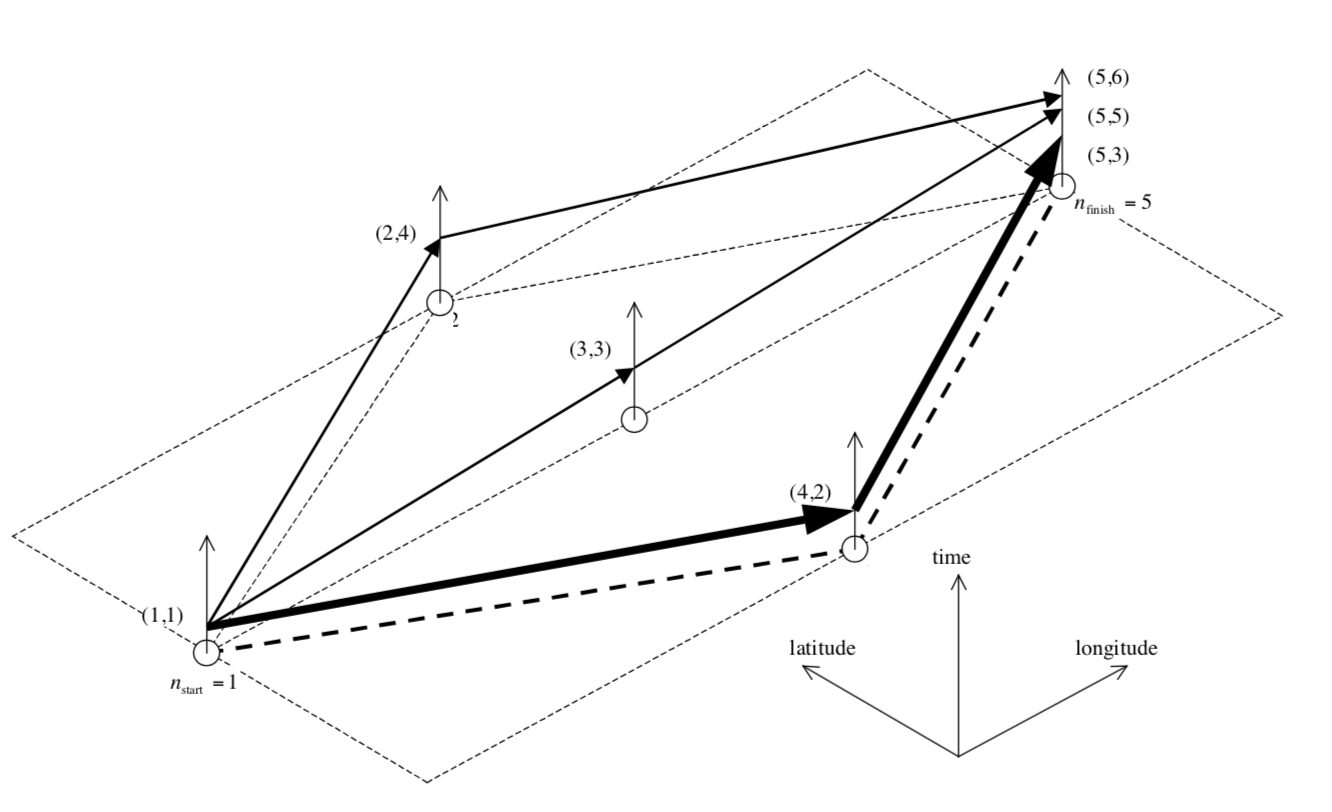
\includegraphics[width=.85 \linewidth ]{Allsopp1.png}
    \caption{Minimal Time Path from node 1 at time 1 (\textit{n(i,t)=n(1,1)}) to node 5 using \acrshort{dp}. The minimal time path to move from node 1 to 5 has go through node 4 and the path is indicated by the thicker  line \cite{allsopp2000optimal}.}
    \label{fig:dp_Allsop}
\end{figure}
\par 

An alternative process to discretize the area is based on the grid method and the heading decision, which is driven by the maximum velocity of the sailboat. This method can be related with the \acrshort{vmg} criterion because the same distance from the starting point can be reached at different times. Here, the heading-angle decision is discretized by intervals of size $\Delta \Psi$, clockwise and counterclockwise as a result multiple sub-routes are generated. If the symmetry of the \acrshort{vpp} is taken into account, some nodes and sub-routes can be represented within a diamond shape \cite{xing2012path} \cite{zyczkowski2017method}. \par \noindent
The number of stages($n_{stages}$) along the straight sailing distance (\textit{L}) between point $P_{0}$ and $P_{n}$ determines the shortest distance between (\textit{L} $\backslash n_{stages}$ ). In this case $n_{stages}$ can have any value bigger than 1 and it can be seen as the number of attacks that the seamanship could perform. The bigger the number the longer the time of the computational effort to determine the trajectory of the optimal time path \cite{xing2012path}. \par 
\noindent
The optimal heading is finding when the next stage is reached at the minimal time. In this case it is possible that multiple nodes arrive at the same time to the next stage. For this reason, the sub-routes have to been stored and the process continues until the destination point is reached. The algorithm to estimate the minimal time path is similar to the $c_{arc}$ process, the difference is in the from in which the area and stages is determined. The heading-direction approach sometimes uses additional factors over directions where the speed is the maximum. \par

Figure \ref{fig:diamondshape_subR} shows how the heading decision works. In this particular case, e all the sub-routes from $P_{0}$ to $P_{n}$ are contained into a diamond shape. Each node is describe by the stage and the node-number per stage, $P n_{stage},i_{sub-route}$ which is determined by the size of $\Delta \Psi$. The nodes over the edges of can only reach the half of nodes compared with the nodes at the center. The number of clear stages represented here are 6 and on each node there a maximum number of sub-routes is 21 and a minimum of 10. It is importance to remember here the concept of the \textit{no-go-zone} from section \ref{sec:VPP} because it could reduce the range of the heading direction angle.\par 

%\begin{figure}[hbt!]
%\centering
%  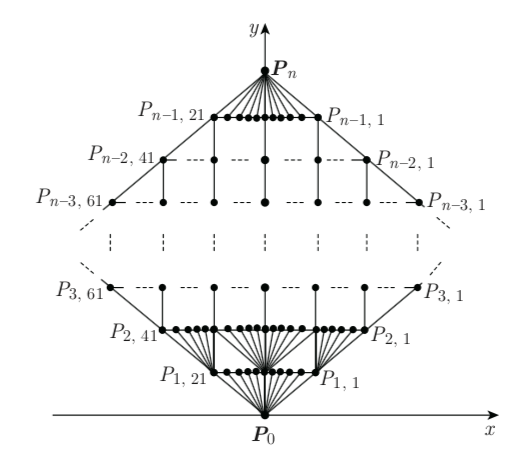
\includegraphics[width=0.6\linewidth]{legyachtxing.png}
% \caption{Leg yatching model \cite{xing2012path} }
%\label{fig:xing_nodesi}
%\end{figure}

\begin{figure} [hbt!]
  \centering
  \subfloat[Sailing Area Discretization for a Sailing Path from point A to B \cite{zyczkowski2017method}.]
  {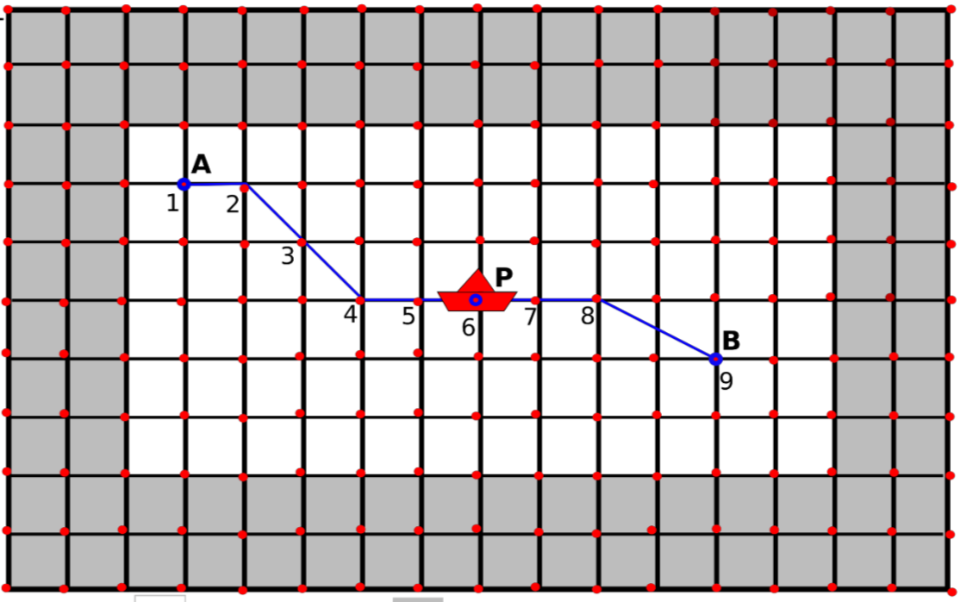
\includegraphics[width=0.33 \linewidth]
  {Sailing_area_heading.png}\label{fig:GridAreaSail}}
  \hfill 
  \subfloat[Heading Directions at a node, 8 angle discretizations \cite{zyczkowski2017method}.]{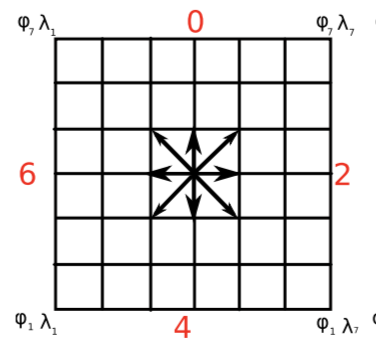
\includegraphics[width=0.22\hsize]
  {HeadDirNode.png} \label{fig:HeadAngle_Discret}}
  \hfill
  \subfloat[Diamond Shape with the Sub-routes for a heading-angle discretization to move from $P_{0}$ to $P_{n}$ \cite{xing2012path}.]
  {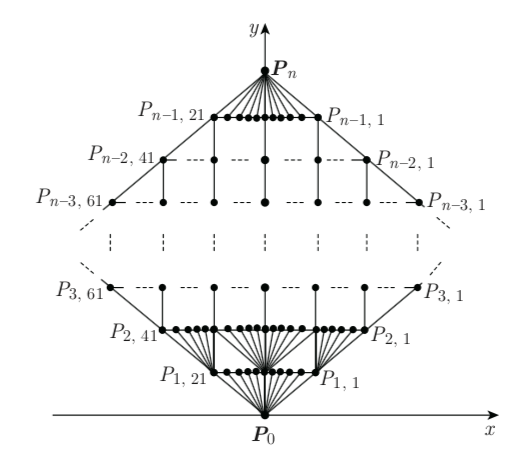
\includegraphics[width=0.33 \linewidth]{legyachtxing.png}
  \label{fig:diamondshape_subR}}
  \caption{Area discretized with a sailing path and Heading Angle discretization}
\label{fig:AreaDiscret} 
\end{figure}

\subsection{Path Algorithm Using Isochrones} \label{sec:isochrones}
A common solution with visual information obtained with \acrshort{dp} in weather routing are the isochrones. The isochrones lines compose a map where each line shows the maximum distance a sailboat can reach during a certain time. Moreover, this map can be seen as the visual representation of the \acrshort{vpp} over different anisotropic media when the weather variation is minimal \cite{allsopp1998stochastic}. \par 
A similar approach relates this type of solution with geometrical optics more specific with wavefronts. This analogy is because the speed of the wavefront depends on the refractive index of the material \cite{rabaudoptimal}.Figure \ref{fig:isochrone_ex} shows how the \textit{qtVlm} software uses isochrones to determine the optimal path for a generic yacht.\par

\begin{figure}[hbt!]
    \centering
    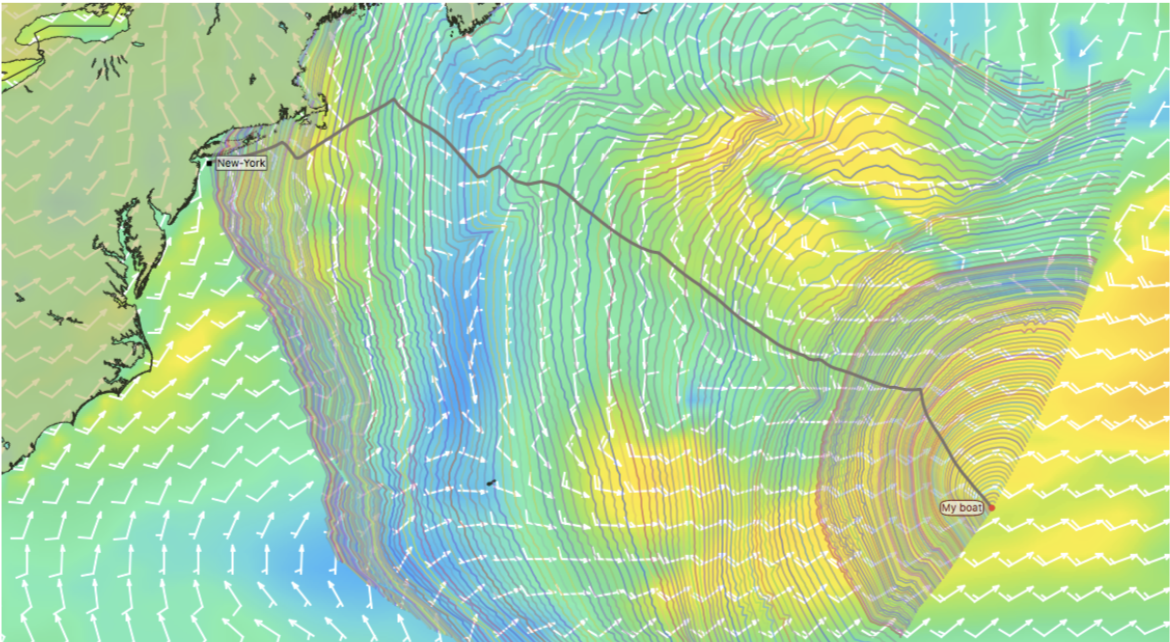
\includegraphics[width=.75 \linewidth]{isochrone_ex.png}
    \caption{Optimal Path Solution from qtVLm software using isochrones for a generic Yacht from a random location over the Atlantic to New York. The optimal path is the gray thick line, the wind direction is indicate by the white arrows.. The \cite{rabaudoptimal}. }
    \label{fig:isochrone_ex}
\end{figure}

The visual information presented by most these algorithms has been employed by various weather routing software. Despite of this, the use of them in sports and in Olympic Sailing Classes is limited. This because they are designed for long-distance yachts races or for maritime-logistics purposes. In both cases, the weather model is assumed to be homogeneous in space and time and frequently loaded from public sources. Meaning that the time step and grid size is much bigger than the required for Olympic Sailing races. Furthermore, when it is used for maritime-logistics purposes the vessels are equipped with communication and other measured systems that accounts for weather variations. \par
Despite the advantages of the isochrones techniques and its usage on large course races, the number of application for short courses is limited. The reason is because the weather is assumed to be perfectly known and even when the \acrshort{vpp} is assumed symmetric the algorithm doesn't explain or shows the limitations of choosing the symmetric path not even as an alternative for some space-time-intervals.\par    

%The envelop shape of the VPP used in \cite{rabaudoptimal} was explained in detail by \cite{dolinskaya2009optimal}.This type of shapes represent a feasible region where a vessel can moves in a straight line in a period of time from the origin; and it was called     \textit{linear path attainable region} for point (0,0)" \cite{rabaudoptimal}.
% resumen 
% points to include use of stages to set the path
% the discretiation of the area, and the wind is assumend location is know
% weather is perfectly know
% alssop interpolation 
% include advantages
\hspace{5mm}
In resume,
%As explained at the beginning of this section
\acrshort{dp} is a flexible method used to find the optimal sailing path and widely used for weather routing. The main characteristics of the previous techniques that have be considered for the development of the laser path algorithm are explained afterward. Before starting any sailing path, first it is important to define the area within any path might take place. This is not only because of the wind or current model but because inside that area a set of stages have also to be defined. This area for the sailing path have to cover effectively all the alternatives so the minimal time path can be found. \par 
After the area is defined it has to be discretized, the grid approach is commonly used. By using the grid it is easy to locate the node for either the node or the arc and to find the value for both wind and current. The discretization is directed related with the granularity of the problem and at the same time with the computational effort. \par 
The next characteristics to define is the number of stages is a free number that must be taken with care. The number of stages in combination with the number of variables define the state-space vector. This vector has to been estimated and later on compared as many arcs or nodes were determined. As a consequence of the size of the vector the computational effort can be affected and at this point the number of operations could grow exponentially.

\section{Adapting the Yacht Model to the Laser Class} \label{sec:laser_yacht}

Most of the research either for path planning or for the physic model for sailboats are related with yacht or with bigger boats such as sailing vessels. Figure shows the differences on heights for the mast only, where a the AC45 yacht race has a height of 25.5 m while the Laser Olympic class mast's height is 6.1 m. Equations on section  \ref{sec:eq_of_motion} are generic an applicable to any kind of sailboat. Hence to represent properly the laser class some modifications have to made before to properly represent its motion.\par 
\begin{figure} [hbt!]
    \centering
    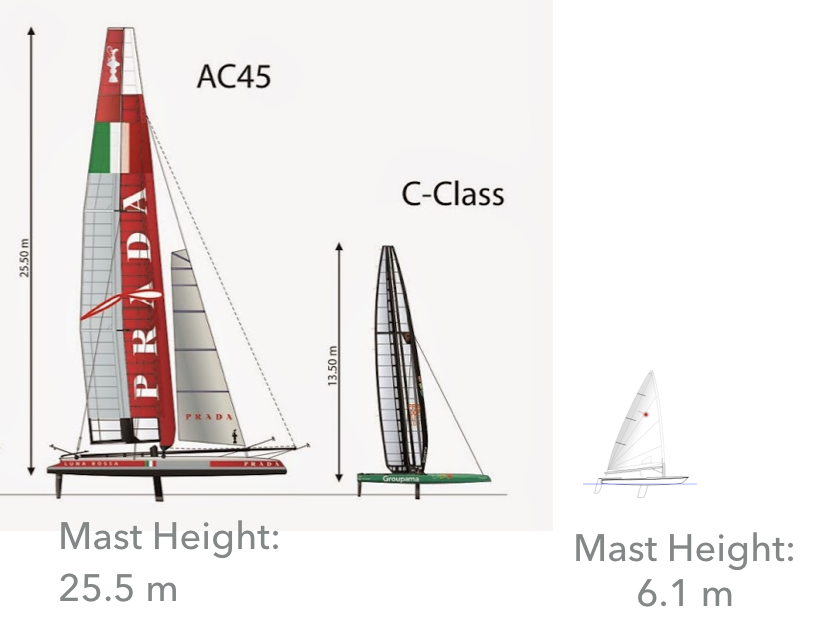
\includegraphics[width=0.75 \linewidth]{yacht_comp.png}
    \caption{Mast Height Comparison between two yachts models AC45 and C-Class versus the Laser Olympic Class, side view. \cite{yacht_compw}.}
    \label{fig:yacht_mast_height}
\end{figure}
The sailboat of the laser class is the dinghy one of the smallest boats propelled by wind, with a maximum weight of 59 kg \cite{sailoly}. Therefore its balance on the \textit{heave axis} (\acrshort{heave_ax}), between the heel angle (\acrshort{heel_ang}) and righting moment (\acrshort{right_m}) is determined by the ability of the crew to adjust its posture over each side of the boat. The posture of the crew respect to the boat is determined by the wind speed and direction mainly. So it can be said that the crew's posture is a response to the weather variations \cite{marchajaereo1979}.\par 

Even when these assumptions are implicit to keep the sailboat analyses in 2-dimensions and developed the \acrshort{vpp} there's is being some discussion about it \cite{philpott1993yacht},\cite{larsonprinciples}. The discussion are related not only with the posture but also with the impact of crew's mass (\acrshort{crew_m}). Since for Olympics Sailing Races it could represent more than $50 \% $ of the total mass of the sailboat (\acrshort{m})\cite{day2017performance}. These without considering the rate of change of these postures adjustments and the assumption that its centroid (\acrshort{crew_m}) is located in the center of gravity (\acrshort{c_g}) of the sailboat. \par 

A deeper analysis and comparison between the adaptations on the standard \acrshort{vpp} were addressed about the coefficients and forces related with the sails. The comparison of the different coefficients values include the data taken from the Offshore Rating Congress (2013) and the observations made in other works \cite{day2017performance}, \cite{carrico17symp}, \cite{binns2002development}, \cite{flay1996twisted}. Furthermore, these modifications correspond to the addition of the \textit{reef} and \textit{flat} coefficients of the sail. Particularly, they account for the fact that dinghy's sail do not reef against strong winds. As a consequence of this, the drag and lift coefficients must been adjusted during the upwind and downwind course \cite{carrico17symp}. \par \noindent
The adaptations directly related with the 
%were divided according the 
aerodynamic 
%and hydrodynamic 
forces, as a result of the \textit{flat}, \textit{twist} coefficients and the \textit{spill}(\acrshort{spill}) variable 
%were included. 
are showed next. These coefficients model the behavior of the sails and the athlete under strong wind conditions and it includes not only the upwind conditions but also the downwind course \cite{day2017performance}. % in additions to some conditions to be included when a downwind course is sailedIn \cite{day2017performance}. \par 
Therefore, equations \ref{eq:Cd} and \ref{eq:Ct} are modified to account the required adjustments. \par \noindent 
Then \acrshort{spill} modifies equation \ref{eq:Ct} and is shown in equation \ref{eq:liftMod} where \acrshort{Ctwist} has a value of  \textit{8.0} and \acrshort{twist} which is the \textit{twist variable} has a range value of [0,1], \acrshort{CDv} and \acrshort{CLmax} is obtained by interpolation from tabulated values and it depends on \acrshort{b_aw} while \acrshort{CDs} has a value of \textit{0.005} and \acrshort{ARE} is based on the rig geometry and calculated according it \cite{day2017performance}. \par \noindent  
Equation \ref{eq:Cd} is replaced by \ref{eq:draftMod}, the values taken were the smallest with an reduction of the area of 20 \% to consider shielding from the cockpit \cite{day2017performance}.\par 
%The effective aspect ratio ARE is calculated from the geometric aspect ratio based on rig geometry

\begin{equation} \label{eq:liftMod}
    C_{t}^*=C_{Dv}(\beta_{aw}-s)+C_{Dp}+f^2 \cdot C_{Lmax}^2 \cdot (\beta_{aw}-s) \cdot \Big(\frac{1+C_{twist} \cdot t^2}{\pi AR_{E}} + C_{Ds}\Big)
\end{equation}

\begin{subequations} \label{eq:draftMod}
 \begin{align}
  C_{d}^*= 1.075 && \text{for the frontal area} \label{eq:FrontalAreaDraft} \\
  C_{d}^*= 0.954 && \text{for sideways area} \label{eq:SideAreaDraft}
 \end{align}
\end{subequations}

\par 
The literature regarding \acrshort{vpp} for laser boat classes is limited and it is mainly accounted in \cite{day2017performance}, the comparisons made here are only valid for wind speed between  4 and 16 knots, while races are performed up to 25 knots. This range have to be consider in the developed of the algorithm to find the optimal path since it is the velocity of the wind that determines the direction that should be taken in order to maximize the \acrshort{vmg} criterion. \par 

\section{The Optimization Algorithm for the Minimal Time Path}
At this point, all the elements required to define the algorithm for the sailing path have been described. In this section those elements are going to be implemented in a similar order in which they were described. First the parameters of the Laser are going to be described so its \acrshort{vpp} can be estimated, then the area for the sailing race has to be defined and finally how the optimization was setting up and validated. 

\subsection{The Laser Olympic Class}
As mentioned before the Laser sailboat is the smallest class of the Olympics Sailing Classes and it is shown in figure . The dimensions and parameters that describe the laser are regulated by the \acrfull{ilca} and they are showed next in addition to some coefficients previously defined. Figure shows a side view of the Laser Standard and Laser Radial which are Olympic Classes. %For the \acrshort{Asail} and \acrshort{Asail_La} equation is used, where $L_{luff}$ refers to the luff lenght and $L_{foot}$ is the length of the foot, for which the maximum dimensions were used.
%\begin{equation} \label{eq:sail_area}
 %   A_{sail}=0.5 \cdot L_{luff} \cdot L_{foot}
%\end{equation}
\begin{description}
        \item \acrshort{mboat}= 59 [kg] \acrlong{mboat}
        \item \acrshort{Loa} = 4.2 [m] \acrlong{Loa}
        \item Beam = 1.37 [m] Beam width
        \item \acrshort{Tc} = 0.787 [m] \acrlong{Tc}
        \item \acrshort{Asail_La} = 5.76 [$m^2$] \acrlong{Asail_La}
        \item \acrshort{Asail} =  7.06 [$m^2$] \acrlong{Asail}
        \item \acrshort{Ak} = 0.23 [$m^2$] \acrlong{Ak}
        \item \acrshort{Ar} = 0.11 [$m^2$] \acrlong{Ar}
        \item \acrshort{Cdhull} = 0.02 [-] \acrlong{Cdhull}
    \end{description}
\begin{figure} [hbt!]
    \centering
    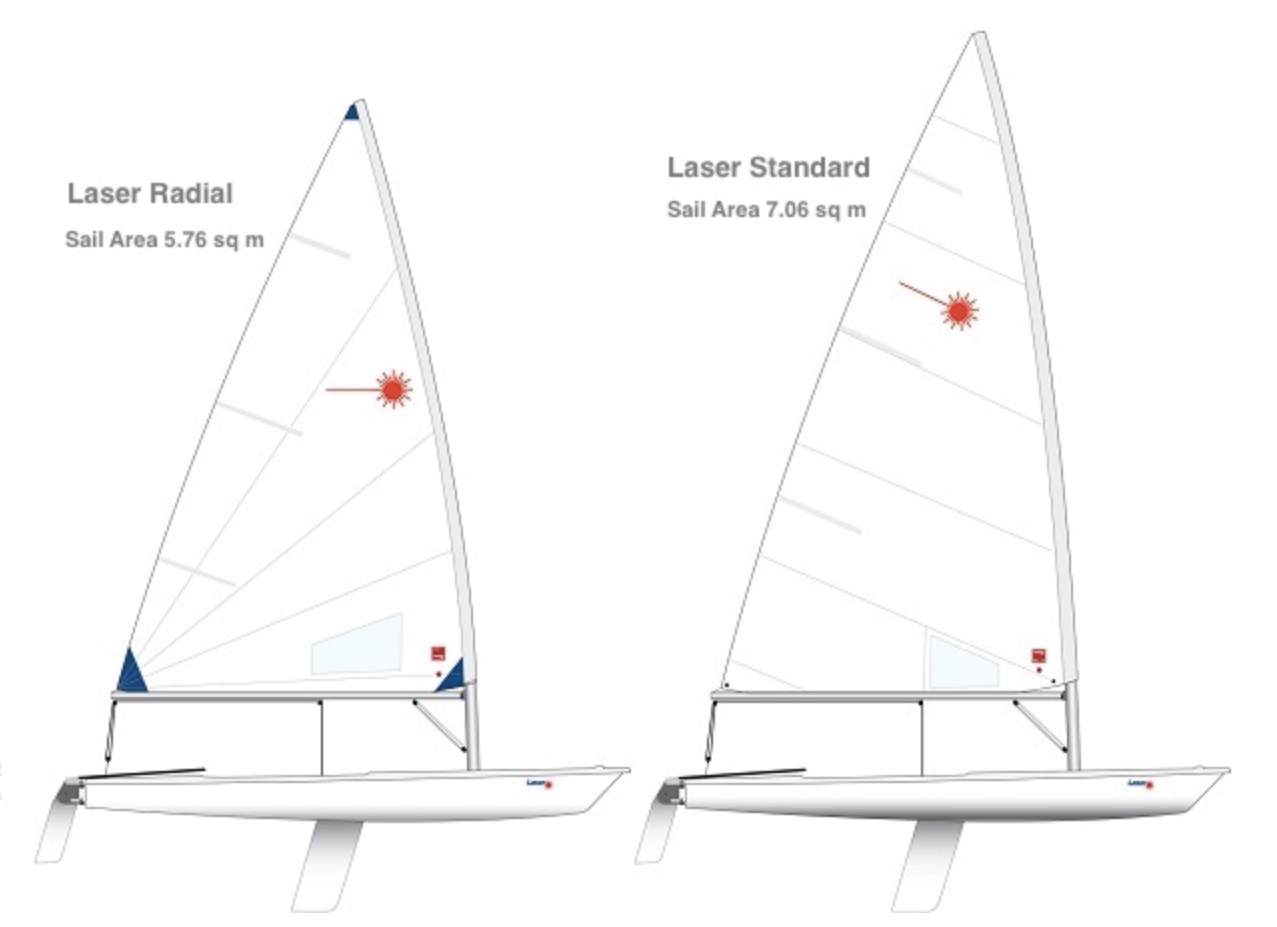
\includegraphics[width=0.64 \linewidth]{LaserOlympicClasses.png}
    \caption{Laser Olympic Classes. Laser standard refers to men category while Laser Radial is for women. The difference between them is only the size of the sail. \cite{2015LaserAssociation}}
    \label{fig:LaserSideView}
\end{figure}
The equations of section \ref{sec:eq_of_motion}, uses the added mass over each axis which according \cite{keuning2004mathematical} can be determined by equations \ref{eq:mx_add} and \ref{eq:my_add}. At this point the \acrshort{crew_m} is required and for the purposes of this research the maximum value suggested by \cite{laser_opt} is used. 
\begin{equation}\label{eq:mx_add}
    m_{x}=2\frac{T_{c}} {Loa} m_{T}=2\frac{T_{c}} {Loa} (m_{boat} + m_{c})=2\frac{0.787}{4.2}(59+70)=48.34 \text{ kg}
\end{equation}
\begin{equation} \label{eq:my_add}
    m_{y}=0.25 \cdot m_{T}=0.25 \cdot (59+70) = 32.25 \text{ kg}
\end{equation}

Most of the coefficients used on the equations of section \ref{sec:eq_of_motion} can be found on tables, however they can be approximate by using sine and cosine functions \cite{rein2012tra},\cite{moreira2011guidance}. These coefficient approximations are referred to the keel ($C_{i,keel}$) and rudder ($C_{i,rudde}$) only and they are shown next, the sub-index \textit{L} is for the \textit{lift} while \textit{D} is for the \textit{drag}. \par 
\begin{subequations} \label{eq:keel_coeff}
    \begin{align}
        C_{L,keel}=0.615sin(2\beta_{k_{a}})+0.025 \label{eq:keel_Liftcoeff}\\ 
        C_{D,keel}=-0.55cos(2\beta_{k_{a}})+0.55 \label{eq:keel_Dragcoeff}
    \end{align}
\end{subequations}
\begin{subequations} \label{eq:rudder_coeff}
    \begin{align}
        C_{L,rudder}=0.6175sin(2\beta_{r_{a}})+0.0325 \label{eq:rudder_Liftcoeff}\\ 
        C_{D,rudder}=-0.55cos(2\beta_{r_{a}})+0.55 \label{eq:rudder_Dragcoeff}
    \end{align}
\end{subequations}
Due to these approximations equations \ref{eq:Side_force}, \ref{eq:att_r} and \ref{eq:att_k} are modified and facilitate the separation of the \textit{lift} and \textit{drag} forces to use them. The angle of attack (\acrshort{a_a})is related with the \acrshort{b_aw}, therefore it is related with the trim angle of the sail (\acrshort{trim_sail}). The keel is a fix element and it is assumed rigid then its \acrshort{b_k_a} is the same as the \acrshort{b_ac}.   \par \noindent %The approximations related to the sail will not be used since equations \ref{eq:draftMod} and \ref{eq:liftMod} 
\begin{equation} \label{eq:app_current_ang}
    \beta_{ac}=atan2\frac{v}{u}
\end{equation}
\begin{equation} \label{eq:app_current_vel}
    V_{ac}=\sqrt{u^2 + v^2}=V_{boat}
\end{equation}
\begin{equation} \label{eq:keel_lift}
    F_{L,keel}=\frac{1}{2} \cdot \rho_{w} V_{ac}^2 A_{keel}C_{L,keel}(\beta_{ac})
\end{equation}
\begin{equation} \label{eq:keel_drag}
    F_{D,keel}=\frac{1}{2} \cdot \rho_{w} V_{ac}^2 A_{keel}C_{D,keel}(\beta_{ac})
\end{equation}
\begin{equation} \label{eq:angle_attack_rudder}
    \beta_{r_{a}} = \beta_{ac} - \delta_{r}
\end{equation}
\begin{equation} \label{eq:rudder_lift}
    F_{L,rudder}=\frac{1}{2} \cdot \rho_{w} V_{ac}^2 A_{rudder}C_{L,rudder}(\beta_{r_{a}})
\end{equation}
\begin{equation} \label{eq:rudder_drag}
    F_{D,rudder}=\frac{1}{2} \cdot \rho_{w} V_{ac}^2 A_{rudder}C_{D,rudder}(\beta_{r_{a}})
\end{equation}
\begin{equation} \label{eq:angle_attack_sail}
    \alpha_{a} = \beta_{aw} - \delta_{sail}
\end{equation}
The motion of the sailboat is dominated by the wind and this research is focus on the effects of the wind. As a result, the $\beta_{i_{a}}$ of the rudder and keel are treated as one component and substituted by $\alpha_{a}$ \cite{rein2012tra}. The implication of this substitution has two effects, first on the \acrshort{Rhull} and second on the lateral force. The coefficient related with the \acrshort{Rhull} has to account for thus it has to increase to \textit{0.025}. \textbf{The lateral forces is assumed to be in equilibrium all the time as a result, the \acrshort{v} velocity known as drift speed is neglected} hence equation \ref{v_dot} is omitted from the equations of motion for the Laser Class \cite{rein2012tra}.\par  
Another modification is related with equation \ref{eq:u_dot} which has to be modify to replace the hydrodynamic derivative expression ($X_{V\psi}$) by a damping expression showed on equation \label{eq:u_dotLaser}. The damping expression is related with a constant value  (\textit{Cnst}) of 0.3 according to \cite{rein2012tra}. \par
\begin{equation} \label{eq:u_dotLaserM}
    \Dot{u}=\frac{X_{TOT}}{m+m_{x}}-Cnst \cdot \Dot{\psi}^2
\end{equation}
To recapitulate all the previous changes, the equations of motion that describes the motion for the Laser Olympic Class are: \par 
\begin{equation} \label{eq:X_uM}
    X_{U}=\frac{1}{2}\rho_{w}V_{boat}^2 \cdot C_{D,hull}=\frac{1}{2}\rho_{w} \cdot V_{ac}^2 \cdot 0.025 
\end{equation}
\begin{equation}\label{eq:X_sailM}
       X_{sail}=F_{L,s}sin\beta_{aw}-F_{D,s}cos\beta_{aw} 
\end{equation}
\begin{equation}\label{eq:Forces_M} 
     X_{current}=m\cdot V_{boat} \Dot{\psi}= m\cdot V_{tc}^b \cdot \Dot{\psi}
\end{equation}
\begin{equation}\label{eq:X_TOTM}
    X_{TOT}=X_{U}+X_{sail}+X_{current}
\end{equation}
where:
\begin{equation} \label{eq:SailLiftM}
    F_{L,s}=\frac{1}{2}\rho_{a}V_{aw}^2 \cdot A_{s} C_{t}^*
\end{equation}
\begin{equation} \label{eq:SailDragM}
    F_{D,s}=\frac{1}{2}\rho_{a}V_{aw}^2 \cdot A_{s} C_{d}^*
\end{equation}
Finally the equations that describe the motion are:\par
\begin{equation}\label{eq:x_dotM}
\Dot{x}=u \cdot cos\phi + u_{tw} + u_{tc}
\end{equation}
\begin{equation}\label{eq:y_dotM}
\Dot{y}=u \cdot sin\phi + v_{tw} + v_{tc}
\end{equation}
\begin{equation} \label{eq:u_dotLaserMR}
    \Dot{u}=\frac{X_{TOT}}{m+m_{x}}- 0.3 \Dot{\psi}^2
\end{equation}

These modified equations serves only for the laser Olympic class and with them the \acrshort{vpp} can be estimated. Even so, at some wind velocities  %the approximations of 
equation \ref{eq:liftMod} %and \ref{eq:keel_coeff}
could be less accurate, specially at \acrshort{v_tw} close to 20 kn and above it. Since equations \ref{eq:liftMod} and \ref{eq:draftMod} work fine when the \acrshort{v_tw} is close to 10 kn \cite{day2017performance}, which is at the lower range of the \acrshort{v_tw} range defined by \cite{laser_opt}. \par 

\subsection{ VPP for the Laser Olympic Class}
The optimization of the minimal time path as showed in equation \ref{eq:rabaudmintime} requires to determine first the velocity which in this case \acrshort{v_aw}($\psi$). \acrshort{v_aw}($\psi$) is related with the wind speed and direction and considering the computational effort and the fact that the wind model is space and time discretized. The \acrshort{vpp} can be estimated first since the wind speed range rule ([4,25]kn) conditions the laser races. To estimate the \acrshort{vpp} not only the \acrshort{b_tw} but also the \acrshort{v_boat} has to be discretized with small steps values. \par \noindent 
Using the previous equations and replaced in equations from \ref{eq:X_tot} to \ref{y_dot} the \acrshort{vpp} can be obtained using an optimization method. The systems of equations can be solve over the angle range of [0,180 \degree] using the built-in function of \textit{fmincon} from \acrshort{matlab}\cite{rein2012tra}. The problem is defined as maximization of the \acrshort{v_boat} which means that all the forces are in equilibrium. However, any  optimization problem has to be defined in terms of the minimum value so the problem is defined as:
\begin{align}
    \text{minimize:}\qquad & -u(u,\psi,\delta_{s},V_{tw})  \label{eq:max}\\
\text{subject to:} \qquad & X_{TOT}=0 \\
 \qquad & Y_{TOT}=0
%& \Dot{v}=0 \\
%& \Dot{\psi}=0
\end{align} \label{eq:opt_vpp2}
instead of: 
\begin{align}
    \text{maximize:}\qquad & u(u,\psi,\delta_{s},V_{tw})  \label{eq:max2}\\
\text{subject to:} \qquad & \Dot{u}=0 \\
%& \Dot{v}=0 \\
& \Dot{\psi}=0
\end{align} \label{eq:opt_vpp}
Equation \ref{eq:max} shows that \acrshort{u} is the boat's velocity and it depends on itself which means that the system is not linear. Moreover, its influence on \acrshort{b_tw}, \acrshort{v_aw} determines the sail's forces. The control variables this problem are $\Dot{\psi}$ and \acrshort{trim_sail}, this last could have a value over the range of [0,180 \degree] but it should not cancel $\Psi$, during motion.
\par
\begin{figure}[hbt!]
    \centering
    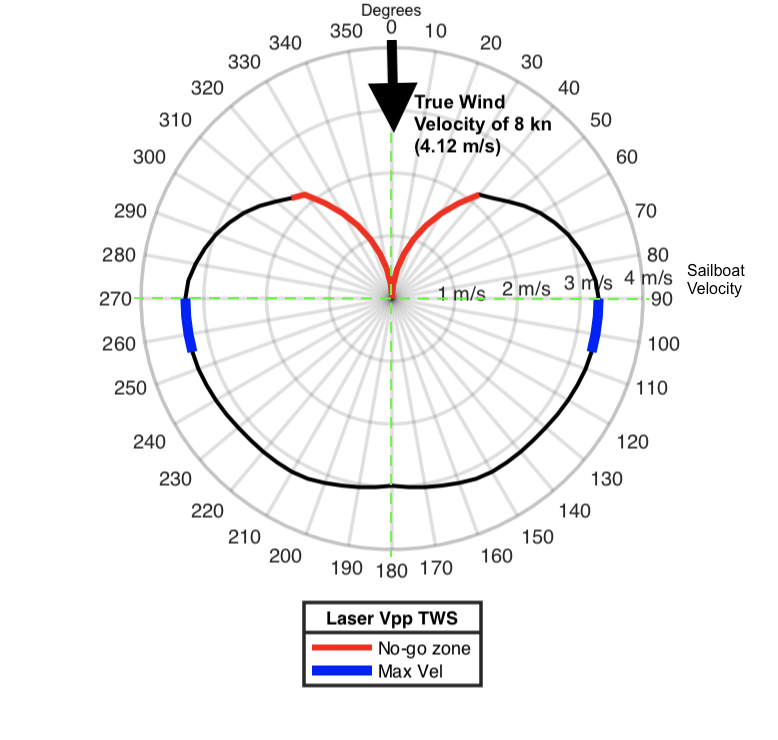
\includegraphics[width=.53 \linewidth]{Vpp_8.png}
    \caption{Full VPP for the Laser Class at 8 kn $V_{tw}$ coming at $0\degree$ from the North, the angles were discretized with and interval of $10\degree$} 
    \label{fig:Laser_Full_Vpp85}
\end{figure}
Figure \ref{fig:Laser_Full_Vpp85} shows the full \acrshort{vpp} of the Laser Olympic Class for a wind of 8 kn. In this graphic the direction of the wind is zero degrees from the North. The angle's interval is $10\degree$ and the \acrshort{v_boat} is indicated by the diameter of the circles in this case, it has a range value of [0,3.3] m$\backslash$s . In the figure the \textit{no-go-zone} is in the angle range of [0, 40] degrees and [320, 360] degrees while the maximum velocity of the boat can be reach in the angle range of [90, 115] degrees and [255, 270] degrees. \par 
\noindent
The \acrshort{v_boat} range taking out the \textit{no-go-zone} is [2,3.3] m$\backslash$s, the \acrshort{vpp} shape over the range of [90,270] degrees does no varies to much. The shape is close to a semi-circle, this means that under a downwind condition a straight trajectory could be more efficient if the tack loss time is bigger than the velocity change ratio while the \acrshort{v_tw} remains constant.  \par  

An alternative method to estimated the half of the  \acrshort{vpp} uses wind measurements for the speed and its direction. These measurements however does not have a constant interval, so to predict any other wind speed and its direction, the measured data is interpolated  
%Interpolating between known values can then give predicted maximum speeds for any true wind angle and true wind speed
\cite{philpott2001optimising},\cite{allsopp2000optimal}. For the purpose of this project, some wind measurements for wind speed  were provided by \acrlong{sailctr}. \par \noindent 
The interpolation used for the missing points was the \acrfull{pchip} from \acrshort{matlab}. The use of this data not only serves as validation for the \acrshort{vpp} calculations but also as data source. This because many of the research regarding \acrshort{vpp} for the Laser Olympic Class only cover a wind speed range of [9,12] kn \cite{day2017performance} and the measurements provided are out of this range and they are shown in figure \ref{fig:hvpp_MeasData}.\par \noindent
Figure \ref{fig:hvpp_MeasData} indicates the measurements taken with black asterisk, the rest of the points, therefore the line is the result of the \acrshort{pchip} interpolation. The wind measured are referred as \textit{TWS} and it is assumed to comes from the North, top of the graph. The \acrshort{vpp} is assumed to be symmetric and due to this, the measurements where only taken in the range of [0,180] degrees. \par 
\begin{figure} [hbt!]
    \centering
    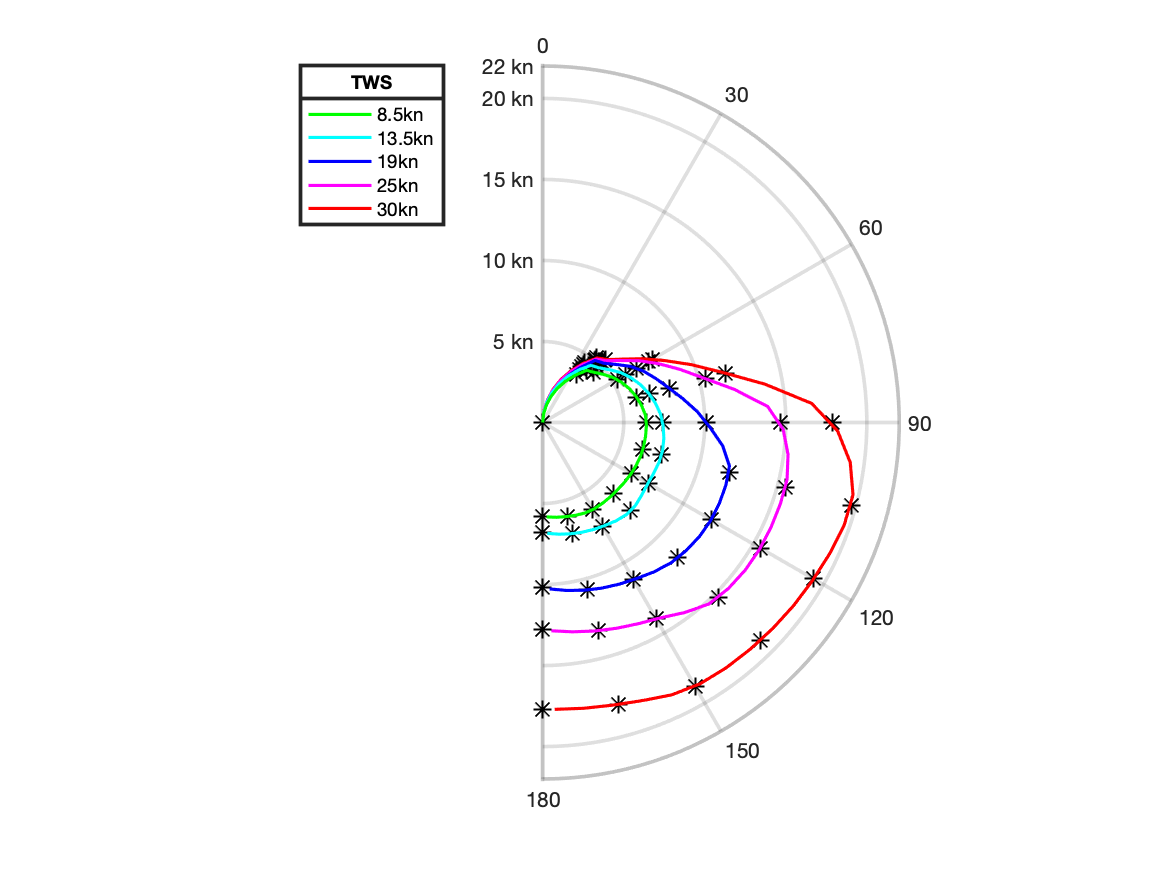
\includegraphics[width=0.72 \linewidth ]{Half_Vpp_laser2.png}
    \caption{Vpp developed with measurements provided by $InnoSportLab\textsuperscript {\textregistered}$, The Hague. The measurements are indicated with black asterisk. The results of the interpolation varies according the wind velocity (TWS)}
    \label{fig:hvpp_MeasData}
\end{figure}
The measured data not only serves to develop the \acrshort{vpp} but also to validate some of the assumptions previously made. Now that the\acrshort{vpp} was determined the formulation of the minimal time path for the Laser Sailing Class can be described.  \par 

\subsection{The Objective Function: The Minimal Time Path}
At this point all the elements required to develop the algorithm have been explained. In this section their implementation is going to take place. The objective is to find the path with the minimum time, regardless the type of sailing course. Figure \ref{fig:SailModes_Man}, shows the three types of courses with its main maneuvers and an angle range where they take place. The angle range is not specify since it depends mainly on the \acrshort{vpp} (type of sail boat) and sailor preferences. For example, under a downwind condition, many sailor prefer to follow a straight line rather than a zig-zag pattern.  \par
\begin{figure} [hbt!]
  \centering
  \subfloat[The 3 main modes to sail respect to the wind direction.]
  {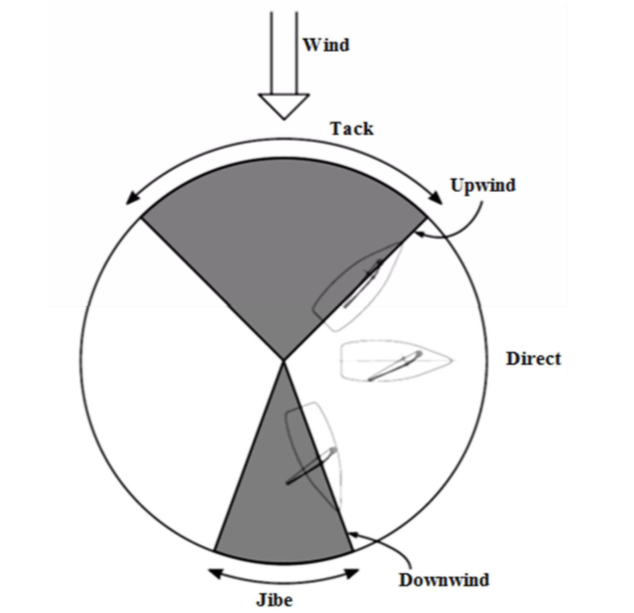
\includegraphics[width=0.45 \linewidth]
  {SailingModes.png}\label{fig:SailModes}}
  \hfill 
  \subfloat[Types of Maneuvers for sailing according the boat and wind direction .]{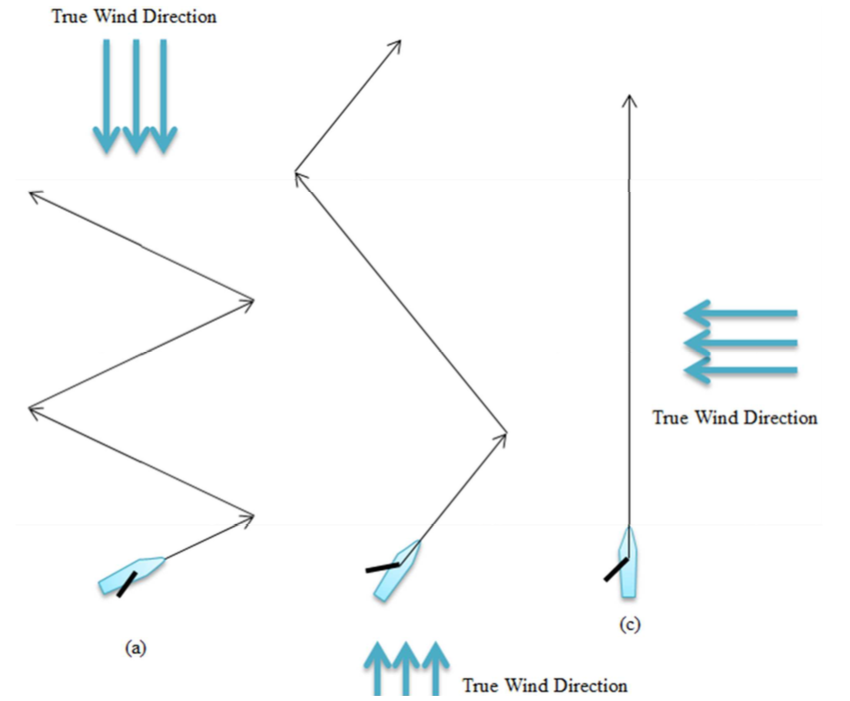
\includegraphics[width=0.5 \linewidth]
  {SailinMAnu.png} \label{fig:maneuversType}}
  \caption{Type of courses and its Maneuvers \cite{Alves2014ASailboat}}
\label{fig:SailModes_Man} 
\end{figure}

The combination of at least two of these sail-modes determines a race for Olympic Sailing Competitions. Each sail-mode over the course is defined as \textit{Leg}, them the minimal time for the race is given by the minimal time on each leg. This optimization problem is defined as a multi-phase problem, where each \textit{leg} is the phase of the problem. It is a multi-phase problem not because all the phases are connected but because on each phase different sets of constraints are implemented.\par
Each leg of the course to race is defined by the index \textit{i} and it starts at 1. %, the total number of legs on a race is 5 but this value could change.. 
The number of stages or states of the variables is defined by the index \textit{n} and it can be described as an intermediate points inside each \textit{i leg} where the time and distance are evaluated.  This means that if there are two legs in total and the number of stages is 5, therefore there are twelve stages in total (\textit{$n \times i = (5+ 1) \times 2 = 12$}).\par 
The approach of this problem is based on direction-dependence technique with the heading-angle decision to generate \textit{k} sub-routes. The reason of the \textit{k} sub-routes is to evaluate the symmetry of the \acrshort{vpp} especially at the beginning of the race.
This not only for the upwind mode and \textit{answer the question why start to port is better (or not) than start to starboard}, furthermore to evaluate the straight-line trajectory over the rest of the wind modes. \par \noindent %on the downwind and direct(reach) mode
Consequently \textit{k} is assigned to have \textit{three values}, 1 for the straight-line trajectory, 2 is for the port(left) and 3 is for the starboard (right) start direction. As a note, on the upwind condition the straight-line is not evaluated, nor optimized. Further details about \textit{k} and \textit{n} are given on coming sections of this chapter.\par 
Then the minimal time path for the Olympic Laser races is based on equation \ref{eq:rabaudmintime} and defined as follow.
The objective function is established by equation \ref{eq:minTO} and it is composed by two terms. The first term accounts for the accumulated minimal time up to the previous \textit{i leg} and it stores the  \textit{k,n} state-space variables of the previous legs, as established on equation \ref{eq:CollectPointsTime}.
The second term is the minimal time for the current \textit{i leg} from the \textit{k} sub-route over the \textit{n} stages. \par \noindent 
The time on the second term is determined by the velocity $v_{k,n}$ which depends on its heading-direction, and on the length's trajectory ($dl_{k,n}$). This means that $v_{k,n}$ is  conditioned by equations \ref{eq:C_xvel} and \ref{eq:C_yvel}, and estimated with equation \ref{eq:VelovertheLenght}.
\begin{align}
%\min_{j \in \Gamma_{i}}\\ 
    \text{min } & T=
    %\int_{t_{0}}^{t_{f}} dt=
    L_{k,n}^{i-1}(\Psi,t_{f})+ min \bigg[ \int_{t_{0}}^{t_{f}}  \frac{dl_{k,n}^i}{v_{k,n}^i} \bigg] \quad ,k \in \{1,2,3\} \label{eq:minTO}\\
\text{subject to:} \quad & \Dot{x}=u(\Psi)cos(\Psi) + u_{tw}+u_{tc} \label{eq:C_xvel} \\
\quad & \Dot{y}=u(\Psi)sin(\Psi) + v_{tw}+v_{tc} \label{eq:C_yvel}
\end{align}
where:
\begin{equation}\label{eq:CollectPointsTime}
     L_{k,n}^{*}(\Psi,t_{f})=[x_{k,n}, y_{k,n},t_{f}]^{*}
\end{equation}
\begin{equation}\label{eq:VelovertheLenght}
     v_{k,n}^{*}=\sqrt{\Dot{x}^2+\Dot{y}^2}
\end{equation}
The boundary conditions showed on equations \ref{eq:locIniX}, \ref{eq:locFinX}, \ref{eq:locIniY} and \ref{eq:locFinY} are determined by the leg, particularly by the location of the start buoy and end buoy. These buoys are located over the sailing area and they determine the direction of the boat to follow along with the direction of the wind, to arrive to the next buoy. The location of each buoy is provided in Cartesian coordinates, as explained in \ref{sec:RefFrames}, the latitude-longitude coordinates can be converted to [X,Y] using the \acrshort{matlab} function \textit{deg2utm(Lat,Lon)}. Equation \ref{eq:InitialTime} defines the initial time for the first leg (\textit{i=1}) which is zero. The initial time for the next leg is given by the final time of the previous leg, as shown in equation \ref{eq:FinalTimeLeg}.
\begin{align}
    \quad & x_{k}(0)^i=x_{1}\label{eq:locIniX} \\
    \quad & x_{k}(t_{f})^i=x_{2}\label{eq:locFinX} \\
    \quad & y_{k}(0)^i=y_{1}\label{eq:locIniY} \\
    \quad & y_{k}(t_{f})^i=y_{2}\label{eq:locFinY}\\
    \quad & t_{0}^1=0 \label{eq:InitialTime} \\
    \quad & t_{0}^{i}= t_{f}^{i-1} \label{eq:FinalTimeLeg}
\end{align}
To connect all the legs, and predict the optimal time path for the whole race, the next equations \ref{eq:x_linkC} and \ref{eq:y_linkC}, gives continuity to the path. This continuity helps the algorithm to control the tack maneuver and estimate the tack angle for each leg change.
\begin{align}
    \quad & x^{i+1}(t_{0}^{i+1})=x^{i}(t_{f}^{i})\label{eq:x_linkC}\\
    \quad & y^{i+1}(t_{0}^{i+1})=y^{i}(t_{f}^{i}) \label{eq:y_linkC}
\end{align}
The tack maneuver refers to the change in direction due to a change of a leg, in other words it is a transition maneuver. This transition maneuver or the turn/tack angle is the angle between the end section (stage) of one leg with the start  section (stage) of the next leg and it is constrained by two equations showed as follow and in figure \ref{fig:tackAngL}.\par
\noindent
for the tack to port:
\begin{equation}\label{eq:tackportC}
40\degree < \Psi_{n_{max}-1}^{i}(t_{f}^{i}) -
\Psi_{n+1}^{(i+1)}(t_{0}^{i}) < 130 \degree
\end{equation}
\noindent
and for the tack to starboard:
\begin{equation}\label{eq:tackstarbC}
-130\degree < \Psi_{n_{max}-1}^{i}(t_{f}^{i}) -
\Psi_{n+1}^{(i+1)}(t_{0}^{i}) < -40 \degree
\end{equation}
\begin{figure} [hbt!]
    \centering
    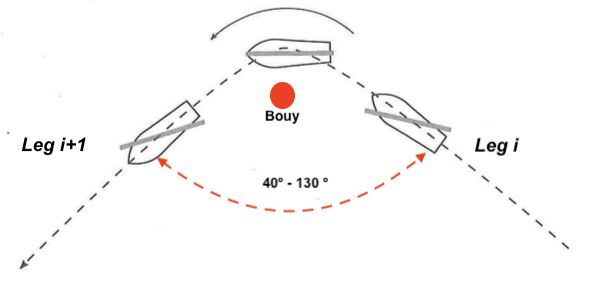
\includegraphics [width=0.55 \linewidth]{tack.png}
    \caption{Tack angle range between legs.}
    \label{fig:tackAngL}
\end{figure}
The final time on each leg is the minimal time and the result of the optimization over that \textit{i leg} and \textit{k} start direction. However, it is known that on the upwind condition, the Laser follows a zig-zag pattern to move against the wind. Moreover, each of these changes in direction takes time and speed and this have to be quantify. For example, \cite{rein2012tra} mentioned a speed loss of 2 kn due to change in direction, other authors refers to these changes as a delay in time of about 5 to 10 seconds before they are reflected in the trajectory \hl{(\textbf{find reference from ch1 and ch2})}. \par \noindent
In this algorithm the number of changes in the trajectory is quantify as a time loss added to the final time on each leg by equation \ref{eq:FinalTime}. The time loss to add of equation \ref{eq:Tot_TimeLoss} depends on the total number of changes in direction during the \textit{i leg}, set on equation \ref{eq:shiftDirCount}, multiple by a constant defined as a $t_{tack-loss}$ and its value is defined in further sections on this chapter. In addition, equation \ref{eq:shift_Dir} controls these shifts in direction so changes larger than 180 \degree  does not happen.
\begin{equation}\label{eq:shift_Dir}
    0 \degree <=\Psi_{k,n+1}^{i}(t_{f}^{i}) - \Psi_{k,n}^{i}(t_{0}^{i}) <180 \degree
\end{equation}
\begin{equation} \label{eq:FinalTime}
    t_{f}^{i}=t_{f}^{*i} + \Delta T_{loss}^i
\end{equation}
\begin{equation} \label{eq:Tot_TimeLoss}
    \Delta T_{loss}^i=t_{tack-loss} \sum_{n=1}^{n} \Delta \Psi_{k}^* (i)
\end{equation}
\begin{equation} \label{eq:shiftDirCount}
\Delta\Psi_{k}^*(i)=
\begin{cases}
0, \quad  \text{if: } \Psi_{k,n+1}^{i}(t_{f}^{i}) = \Psi_{k,n}^{i}(t_{0}^{i})\\
\\
1 %\quad  \text{if: } \Psi_{k,n+1}^{i}(t_{f}^{i}) \neq  \Psi_{k,n}^{i}(t_{0}^{i})\\
\end{cases}
\end{equation}
\begin{equation} \label{eq:TimeFinal_acum}
    t_{f}^{*i}=\sum_{i=1,k}^{i} \Big( t_{f}^{i,k} - t_{0}^{i,k} \Big)
\end{equation}
The state-space limits for the variables are defined in equation \ref{eq:xlox_leg_alt}, \ref{eq:ylox_leg_alt} and \ref{eq:Dirlox_leg_alt}.  The first two limits the position of the sailboat while the last limits the heading angle ($\Psi$) to evades the \textit{no-go-zone}.
\begin{align}
    \quad & x_{min}^{i,1}<x(t)_{n}^{i,1}<x_{max}^{i,1} \label{eq:xlox_leg_alt}\\
   \quad & y_{min}^{i,1}<y(t)_{n}^{i,1}<y_{max}^{i,1} \label{eq:ylox_leg_alt}\\
   \quad & \Psi_{min} <\Psi(t)< \Psi_{max} \label{eq:Dirlox_leg_alt} \\
  \text{where:} \quad & 40\degree  <\Psi(t)< 320\degree \nonumber 
\end{align}
 As mentioned before on each leg the state-space constraints are different, to determined these limits the coordinates of the mid-point of the straight-line trajectory (\textit{k=1}) between buoys is required. The tolerance factor $x_{SAtot}$ and $y_{SAtot}$ determine the minimum and maximum values of the coordinates and defined the limits on each leg. The next equation shows how these estimations are done. In the case of the minimum value or lower bound, it requires the minimum coordinate for \textit{X} and \textit{Y} coordinates from the \textit{3 sub-routes} while for the upper limit it is the maximum of them, in both cases it is also required the $x_{mean}^{i}$ \textit{mean values from the 3 sub-routes (k) }. \par 
 
 The value of this factor should be chosen carefully, one of the reason is that a bigger area not always have more nodes, and the algorithm will take more time to estimate the optimal solution. Moreover it is possible that a local minimum will be find instead of the global solution, because of this it was suggested to run the algorithm several times  guessing some of the initial conditions. The next iterations serves to tune this conditions until they remain the same \cite{philpott1993yacht}. %and changing them for the next time. If the solution remains the same the solution is the optimal, otherwise  
\begin{equation} \label{eq:Xmin_SailArea}
    x_{min}^{i}=x_{mean}^{i} - x_{SAtol}\cdot \Bigg[ x_{mean}^{i} -  min \bigg( x(t_{0}^{i})^{i},x(t_{f}^{i})^{i} \bigg) \Bigg]
\end{equation}
\begin{equation} \label{eq:Xmax_SailArea}
    x_{max}^{i}=x_{mean}^{i} + x_{SAtol}\cdot \Bigg[ x_{mean}^{i} -  max \bigg( x(t_{0}^{i})^{i},x(t_{f}^{i})^{i} \bigg) \Bigg]
\end{equation}
\begin{equation} \label{eq:Ymin_SailArea}
    y_{min}^{i}=y_{mean}^{i} - y_{SAtol}\cdot \Bigg[ y_{mean}^{i} -  min \bigg( y(t_{0}^{i})^{i},y(t_{f}^{i})^{i} \bigg) \Bigg]
\end{equation}
\begin{equation} \label{eq:Ymax_SailArea}
    y_{max}^{i} = y_{mean}^{i} + y_{SAtol}\cdot \Bigg[ y_{mean}^{i} -  max \bigg( y(t_{0}^{i})^{i},y(t_{f}^{i})^{i} \bigg) \Bigg]
\end{equation}

The optimization problem and its constraints for the minimal time path for the Laser Class has been defined. These constraints not only helps the algorithm to get the optimal solution but also to connect all the legs. The connection between legs is made by means of the tack angle, a simplify approach followed for the purposes of this research \cite{jouffroy2009steering}, \cite{LinXiao2011ModelingYachts}.\par 
The state-space constraints are coupled not only withe the wind forecast model but with the course of the competition. Even when some space boundaries varies according to the leg to course, it is the orientation of leg relative to the wind angle the parameter that tune the boundaries of this area. For this reason, a further section will explain how the integration of the curse is made, more precisely the locations of the buoys into the minimal time path trajectory.\par 

% which is simplification approach to acknowledge.    For more details review 
 \subsection{Definition of the Sub-routes (\textit{k=2,3}) at port and starboard direction}

The optimization algorithm initialize with 3 alternative sub-routes and they are defined by the \textit{k} index, moreover, these sub-routes are defined in the same way for any leg. The reason of them is not only because of the heading-angle approach but also because the \textit{fmincon} function from \acrshort{matlab} request initial values of the variables used on the cost function to find the optimal solution of the problem by starting at different points \cite{mitchell2000geometric}, \cite{kelly2015transcription}. \par 

Starting at different points allows the conversion of the solution, however in this case it also aim to the strategy of the race for coaches and athletes. In addition, it aims to limit the area within the optimal path is found and reduces the computational effort also. Because the \acrshort{vpp} has a non-convex shape a path attainable region can be define, the implication of a non-convex \acrshort{vpp} implies that the optimal path may not be unique \cite{dolinskaya2012time},\cite{dolinskaya2013fastest}.  For example, on the upwind condition the maximum velocity is found after the 40\degree, and there are two possible trajectories to follow and reach the next buoy using also the \acrshort{vmg} criterion. \par 
First, at 45\degree the sinus and cosine functions have the same value and it is out of the \textit{no-go-zone}. This means that it possible to sailing at 45\degree respect to the wind direction until the mid-point %on the \textit{X-coordinate} 
and then tack at -45\degree until the target buoy is reached. By doing these tacking maneuvers on both directions port and starboard directions, the sailing area for each leg can be setup. This area can also can be stretching using the $x_{SAtol}$ and $y_{SAtol}$, this is done to give additional space for possible wind shifts, \cite{xing2012path}. \par \noindent
The second alternative is to tack at 45\degree until the target buoy can be reach by making a turn of 90\degree respect to the wind. This alternative was not followed, first because even when the velocity at 90 \degree is the fastest the distance to sail is the larger. Moreover under a constant wind speed and  direction, the ratio between the distance to sail versus the ration between velocities is larger. Therefore, there is no advantage to sail at a higher velocity because the distance to cover does no compensate the increment on the velocity and this only increase the time to reach the target buoy. \par 
\begin{figure}[hbt!]
    \centering
    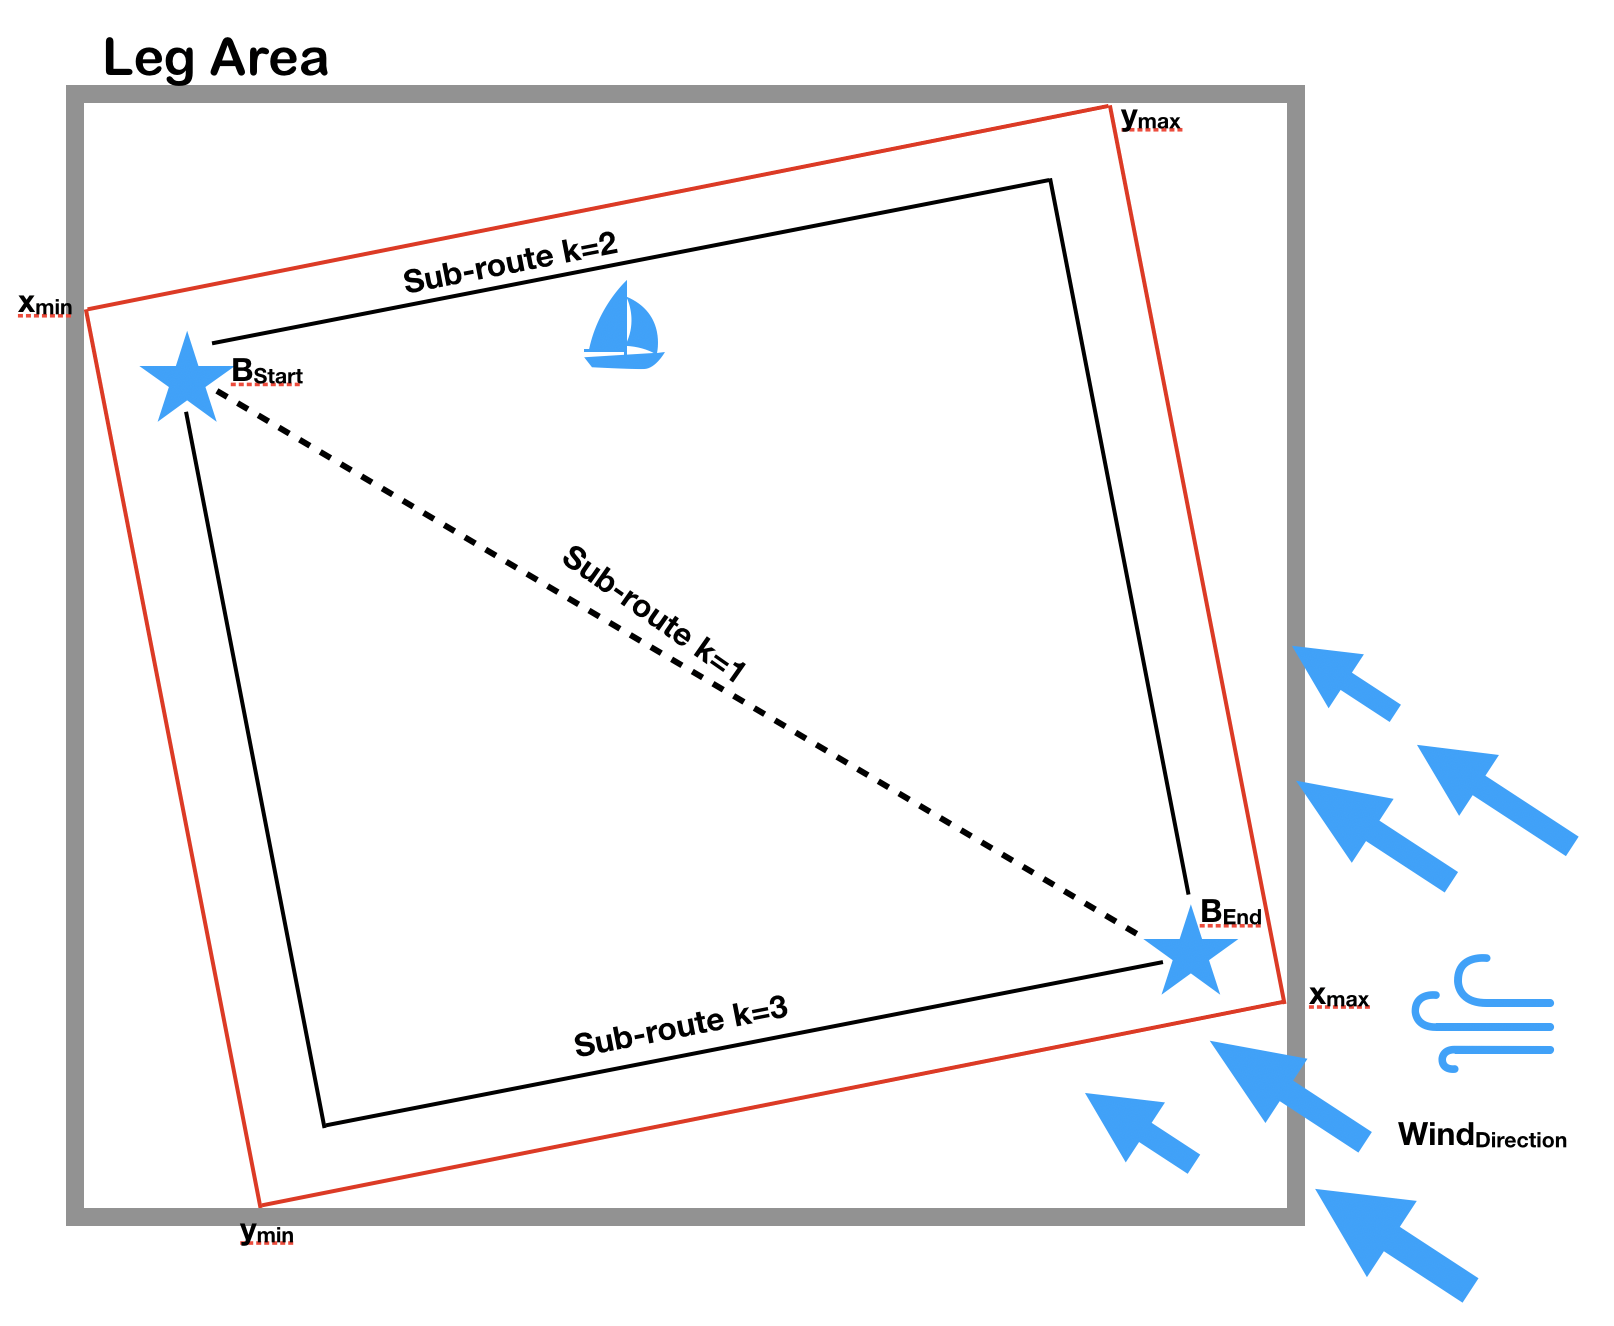
\includegraphics[width=0.5 \linewidth]{LegSail.png}
    \caption{Example of a Sail Area for a Leg using the sub-routes}
    \label{fig:LegSailArea}
\end{figure}
Following the first alternative 2 sub-routes where developed one for the port direction which is assigned by \textit{k=2} and the other to starboard assigned by \textit{k=3}. For the rest of the wind conditions the same approach is followed to define these two sub-routes and therefore the bounds for the sailing area on each leg.  \par
The \textit{n} stages of each sub-route are located within each sub-route so \textit{n} are points defined by \textit{[X,Y]} coordinates and its location determines the path to followed for a particular leg. In addition to this \textit{n} stages, a number of intervals between them were defined to describe properly the $dl_{k,n}^{i}$ of the objective function (equation \ref{eq:minTO}).  This number of intervals and the \textit{n} stages are designated at the beginning of the algorithm and they are part of the initialization parameters a large number for the interval value is recommend to have a smooth path, so the interval is designed by equation \ref{eq:interval}. For example, \textit{9 stages} with \textit{100 intervals} it generates \textit{1010} length elements per sub-route. 
\begin{equation} \label{eq:interval}
   \text{Interval: }  m=100
\end{equation}
\begin{equation} \label{eq:interval-example}
  elements_{dl}=(n+1) \cdot (m+1)
\end{equation}
These sub-routes serves to defined the limits on each leg, not by the means of coordinates of each point but by the maximum and minimum value of those coordinates. The shape of the area for each leg is a rectangle where the coordinates of the opposite corners are defined as equations \ref{eq:Xmin_SailArea}, \ref{eq:Xmax_SailArea}, \ref{eq:Ymin_SailArea} and \ref{eq:Ymax_SailArea} and example of this area is showed in figure \ref{fig:LegSailArea}.\par 
%Because inside each leg numer of \textit{n} st
%The algorithm is build in states (\textit{n}) inside each leg \textit{n}) , along each stage the dl will take place. The reason of this is to control the number of tacks along the leg, and in such way the zig-zag could be define.
\subsection{Course Integration into the Time Optimization Path Algorithm} \label{sec:Coure_LegIntegration}

The setup of the course is defined by the organizers of the event and this is done with the a diagram and with the location of the buoys using \textit{latitud-longitud coordinates}. The importance of them is because the space constraints explained before are linked with the legs of the course which in consequence are related with the buoy's location. The location of the buoys define the distance to sail, the angle direction of the leg respect to the wind direction and as result the wind mode to sail. \par 

An example of the information about the course is showed in figure \ref{fig:Rio_Course1} and it shows a \textit{trapezoid course}, where the start and end of the competitions is defined by a line. In this course there are 6 buoys, 2 line indicator and 2 boats. The letter next to the number of the buoy indicates it locations respect to the boat, so \textit{s} is for \textit{starboard} and \textit{p} for \textit{port}. The order of the marks, indicated in the table below of the diagram, describes how the legs are designated and the code or signal for that sequence. The coordinates of the buoys are provided previous to the race, since they depend on the wind direction and other factors.  \par 
\begin{figure} [hbt!]
    \centering
    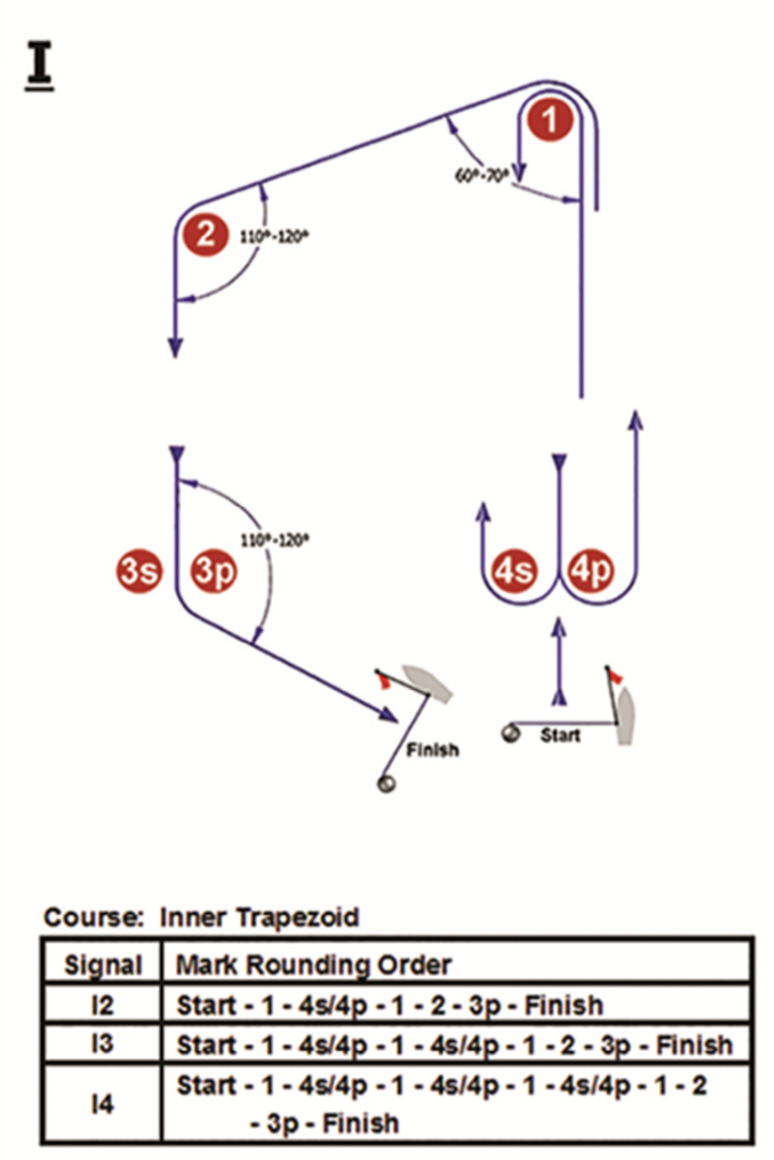
\includegraphics[width=0.39 \linewidth]{course_rio.png}
    \caption{The I Trapezoid Course diagram provided for the Sailing competitions on Rio 2016 Olympics \cite{sailoly}.}
    \label{fig:Rio_Course1}
\end{figure}
For the purposes of this research, the marks where a line is defined or where 2 buoys are designated with the same number, a mid point is going to be calculated to represent this condition. However, for the start and the end line the location of both ends is considered and the mid point is also going to be calculated. The reason of these three points, on the start and on the end line is to account the variation of the wind direction and review how sensible is the time path on the first leg and on the last leg. \par

The location of the buoys most of the time is provided in \textit{latitud-longitud coordinates} and the units are degrees-minutes-seconds, before to convert them to \textit{[X,Y] coordinates} they need to be converted to degrees. This conversion is made using the \textit{dms2degrees} from \acrshort{matlab}. Once this conversion is done, and using the order of the buoys the algorithm will estimate the distance between them with the \acrshort{matlab} function \textit{pdist($b_{1},b_{2}$,'euclidean')}. \par \noindent The angle between them is based on the normal plane, since the wind angle is respect to the \textit{Norht} it is determined in degrees by equation \ref{eq:bouy_angle}, where \textit{i} is the index related to the leg. However, even when this expression only refers to the leg, it can be used to estimate the heading-angle($\Psi$) and  therefore $dl_{k,n}^{i}$. \par 

\begin{equation} \label{eq:bouy_angle}
    \theta_{{i}}=atan2d \bigg [\frac{x_{2}-x_{1}}{y_{2}-y_{1}} \bigg] ^{i}
\end{equation}

The wind mode of the leg is given by the difference between %the angle of the leg 
\acrshort{ang_bouy} %respect to the wind and
and the wind angle, %for now on it is defined as \textit{\acrshort{twd}} instead of 
\acrshort{b_tw}, depending on the difference between those angles the wind mode and its angle are defined by equation \ref{eq:wind_modesDef}. The wind mode angle of the leg (\acrshort{angLegWind}) is defined at the beginning of the competition (\textit{$t_{0}$}), in order to start the calculations of the sub-routes. In this case, %The \acrshort{twd} 
the \acrshort{b_tw} only depends on time in the next section is going to be explained how this value is determined since in section \ref{sec:SailinArea_WindModel} it was explained that it depends on 4 dimensions.\par 
\begin{equation} \label{eq:wind_modesDef}
\Omega_{i,t_{0}} = \mid \theta_{i}-\textrm{TWD}_{t} \mid,
- \quad 
    \begin{cases}
        \text{Upwind(Upw)} \quad &
            \begin{cases}
                0\degree  &\leq  \mid \theta_{i}-\textrm{TWD}_{t} \mid    \leq    45\degree \\
                315\degree  &\leq    \mid \theta_{i}-\textrm{TWD}_{t} \mid  \leq   360\degree \\
            \end{cases} \\ 
    \\
        \text{Direct(Rch)}\quad &
            \begin{cases}
                45\degree   &<     \mid \theta_{i}-\textrm{TWD}_{t} \mid \leq   135\degree \\
                225\degree &\leq \mid \theta_{i}-\textrm{TWD}_{t} \mid <  315\degree \\
            \end{cases}\\
    \\
        \text{Downwind(Dwn)}\quad &
            \begin{cases}
                135\degree &<  \mid \theta_{i}-\textrm{TWD}_{t} \mid <  225\degree \\
            \end{cases}
            
    \end{cases}\\
\end{equation}
The buoys and its orientations respect to the wind define the legs and the limits of the area for each leg using the sub-routes as a reference. The \acrfull{angLegWind} determines the maximum velocity that the sailboat can achieve, once the intensity and location of the boat is known.  Now that the parameters for the course on each leg are defined, the next section will explained how the wind model is going to be integrated into the algorithm. \par 

\subsection{Coupling the Wind Model with the Sail Course} \label{sec:SailinArea_WindModel} %for the Time Optimization Path Algorithm
Until now, the optimization algorithm has been described along with the state-space constraints only in terms of space coordinates. In the other hand, section \ref{sec:WRF_WindM} has described the \acrshort{wrf} wind model in general, while section \ref{sec:WRF_WindM_FR} provide all the details for the model used on this research. To move the sailboat not only it needs a target but also to know the wind velocity \acrshort{v_tw} at a specific time and location.\par \noindent %where is going to be head sailboat from one point to another it the
This section describes how the wind model of section \ref{sec:WRF_WindM_FR} is integrated into this algorithm, so equation \ref{eq:VelovertheLenght} can be determined. The reasons of this integration and adaptation, first, is because the area covered by the \acrshort{wrf} wind model of section \ref{sec:WRF_WindM_FR} is much larger than the area of the course. Second, the time step ($\Delta t$) is about 10 minutes, meaning that the wind characteristics remain constant along this $\Delta t$. However, it is most probably that the space-time dimensions for the estimation of the \acrshort{v_tw} does not corresponds exactly with the space-time coordinates of the grid from the \acrshort{wrf} model despite this its value has to be estimated. \par \noindent Moreover, the time at which the competition starts has to be included during the initialization of the algorithm in addition to the duration of the race and some delays, all this factors are considered for the definition of the \textit{time window}.\par

Previous to the race date, the location of the sail course and the estimated time to start it are known. If the conditions are not meet the race could be delay until this they are meet or in the worst case scenario, the race could be canceled. Because of this, using the start time and the duration of the race (estimated to be about \textit{one hour}). The \textit{time window} is estimated by equations \ref{eq:time_window0} and \ref{eq:time_windowf} adding a bonus time or tolerance up to \textit{three hours} for the upper limit and subtracting \textit{two hours} for the lower limit.

\begin{align} %
    \textrm{Time window} &=\big[\textrm{Time window}_{0},  \textrm{Time window}_{f} \big]\label{eq:time_window}\\
    \textrm{Time window}_{0}&=\textrm{Time start}_{floor}-\textrm{Lower Tolerance} \label{eq:time_window0}\\
    \textrm{Time window}_{f}&=\textrm{Time start}_{ceil}+\textrm{Upper Tolerance}+\textrm{Duration}_{Race} \label{eq:time_windowf}
\end{align}

The tolerances are not the same for both limits because due to the weather conditions most of the time the competition could be delay rather than changed for and earlier time. In cases where the time is not defined in hours only, the start time is rounded to a \textit{floor} value, while for the end time it is rounded to a \textit{ceil} value. The round or floor value in this case is setup for an integer hour value, but it can be change for half-hour or any other value. For example, if the start time is 13:25 hrs, the time window is:
\begin{align} %\label{eq:time_window}
   \begin{split}
        \textrm{Time window}_{0}&= 13:25\textrm{ hr}_{floor} -\textrm{2 hr}\\ 
        &= 13:00\textrm{ hr} - 2\textrm{ hr}
   \end{split} \label{eq:time_window0Ex}\\
    \begin{split}
        \textrm{Time window}_{f}&=13:25\textrm{ hr}_{ceil}+\textrm{3 hr}+\textrm{1 hr}\\
        &= 14:00 \textrm{ hr} + 3\textrm{ hr} +1 \textrm{ hr} \label{eq:time_windowfEx}
    \end{split}
    \\
    \textrm{Time window} &= \big[11:00,18:00 \big]
\end{align}

The definition of the \textit{time window} helps to reduce the length of the \textit{time dimension} from the \acrshort{wrf} wind model. For example, on section  \ref{sec:WRF_WindM_FR} it was mentioned the size of their dimensions, which are (\textit{x,y,z,t}) 198 $\times$ 301 $\times$ 50 $\times$ 145, since $\Delta t = 10$ minutes. Using the previous example of the \textit{time window}, this means that instead of using the 145 time-datasets only \textit{43} time-datasets are used on this algorithm. This reduces the time of processing for this model since only aprox. $30\%$ of them are used to determine the solution of the minimal time path.\par 

Previous to the competitions, with a couple of months in advance, the location and diameter of the course area is communicated to the participants. Using these information, without any details about the location of the buoys, the area from the wind model for this algorithm is defined as a circle inscribed in a square. The coordinates of the opposite corners of this square are modified as equations \ref{eq:Xmin_WindArea},\ref{eq:Xmax_WindArea},\ref{eq:Ymin_WindArea} and \ref{eq:Ymax_WindArea} indicate. The tolerance of the wind area is determined by the radius of the sail course multiplied by \textit{n} times the grid space  ($\Delta x$) of the \acrshort{wrf} wind model. \par
\begin{equation} \label{eq:Xmin_WindArea}
    X_{W,min}= X_{CTR,course}-\frac{\clock_{course}}{2} \cdot n \Delta x
\end{equation}
\begin{equation} \label{eq:Xmax_WindArea}
    X_{W,max}= X_{CTR,course} + \frac{\clock_{course}}{2} \cdot n \Delta x
\end{equation}
\begin{equation} \label{eq:Ymin_WindArea}
    Y_{W,min}= Y_{CTR,course}-\frac{\clock_{course}}{2} \cdot n \Delta x
\end{equation}
\begin{equation} \label{eq:Ymax_WindArea}
    Y_{W,max}= Y_{CTR,course} + \frac{\clock_{course}}{2} \cdot  n \Delta x
\end{equation}

The value of \textit{n} depends on the size of the grid, $\Delta x $, respect to the \textit{radius} of the course as indicated in equation \ref{eq:n_windTolerance}. Since the  \cite{race_pol2017} establishes that the trapezoid course must be contained in this area, so \textit{n} is the next integer value from the ratio between them. If the coordinates of the buoys are known, the minimum and maximum value of all of them are used instead of the coordinates of the center of the sail area to define the corners of the wind area. \par % and the limits for the wind model are defined in a similar way. \par 
%\begin{equation}\label{eq:WRF_windArea}
%\end{equation}
\begin{equation} \label{eq:n_windTolerance}
    n=\lceil \frac{\clock_{course}}{2 \cdot \Delta x}
\end{equation}
%\begin{equation} \label{eq:TolWindArea}
%2\cdot \Delta x =
%\begin{cases}
%\Delta x \textrm{,} \quad & \Delta x < 1000\\
%\Delta x\textrm{,} \quad & \Delta x 
%\end{cases}
%\end{equation}

Using the previous equation the wind area is defined for this algorithm and it is larger than the area of the course, figure \ref{fig:WindAreaSketch} sketch this concept. It shows that if the center of the sail area is sufficiently far for any grid data-point, for example, within a sail of area with a $\clock = 3 \Delta x$ it only contains \textit{four} data-points while within the wind area defined with the previous equations it contains 64 data-points.\par

It is important that regardless the location or time, the algorithm should be capable to estimate the wind's velocity. % at any time and location. 
Particularly when the coordinates are not coincident with those of the grid from the wind model. Thus to estimate the velocity at any point over the space and time an interpolation method is required. The data-points around the point of interest must be enough to estimate this value, moreover the area defined for the wind.  \par 
%For example, %if the location is close to the limits of the sail area, the available datapoints are sufficient and the interpolation can be made without compromising 

\begin{figure} [hbt!]
    \centering
    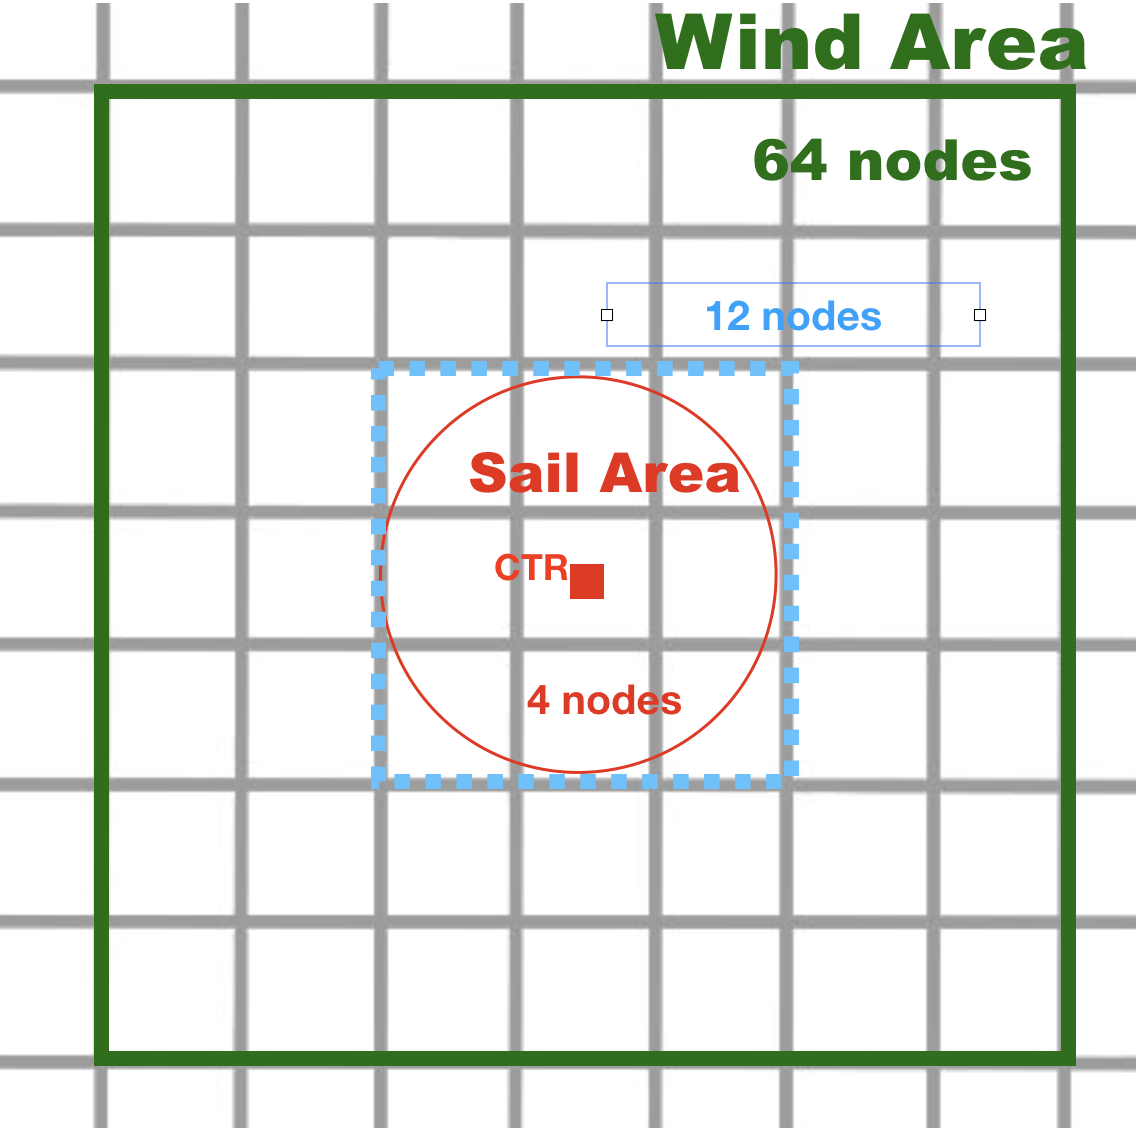
\includegraphics[width=0.32 \linewidth ]{gridWind.png}
    \caption{Wind Area Concept using a wind model representation. The inscribed sail area shows the limits of the square and its corners are used for the definition of the wind area.}
    \label{fig:WindAreaSketch}
\end{figure}

The interpolation method used in this algorithm is the \textit{griddata} function from \acrshort{matlab}. This function-method estimate the components of the wind's velocity %($u_{tw}$ and $v_{tw}$) at any time and position 
using the coordinates from the grid arrangement of the \acrshort{wrf} wind model. Figure \ref{fig:gridDataInterpo} shows a graphical representation of how this function and the wind model interacts. It shows how two datasets for the velocity with coordinates \textit{[X,Y,t]} are used to determine the velocity $V_{tw}^{*}$ at $t^{*}$ which is intermediate from $t_{0}$ and $t_{1}$. Inside the function to obtain the requested value, a method has to be defined in cases where a liner interpolation doesn't apply. %for the interpolation of the values 
For the velocities, in this research, the \textit{nearest} option for the method is used inside the \textit{griddata} function.\par

\begin{figure}[hbt!]
    \centering
    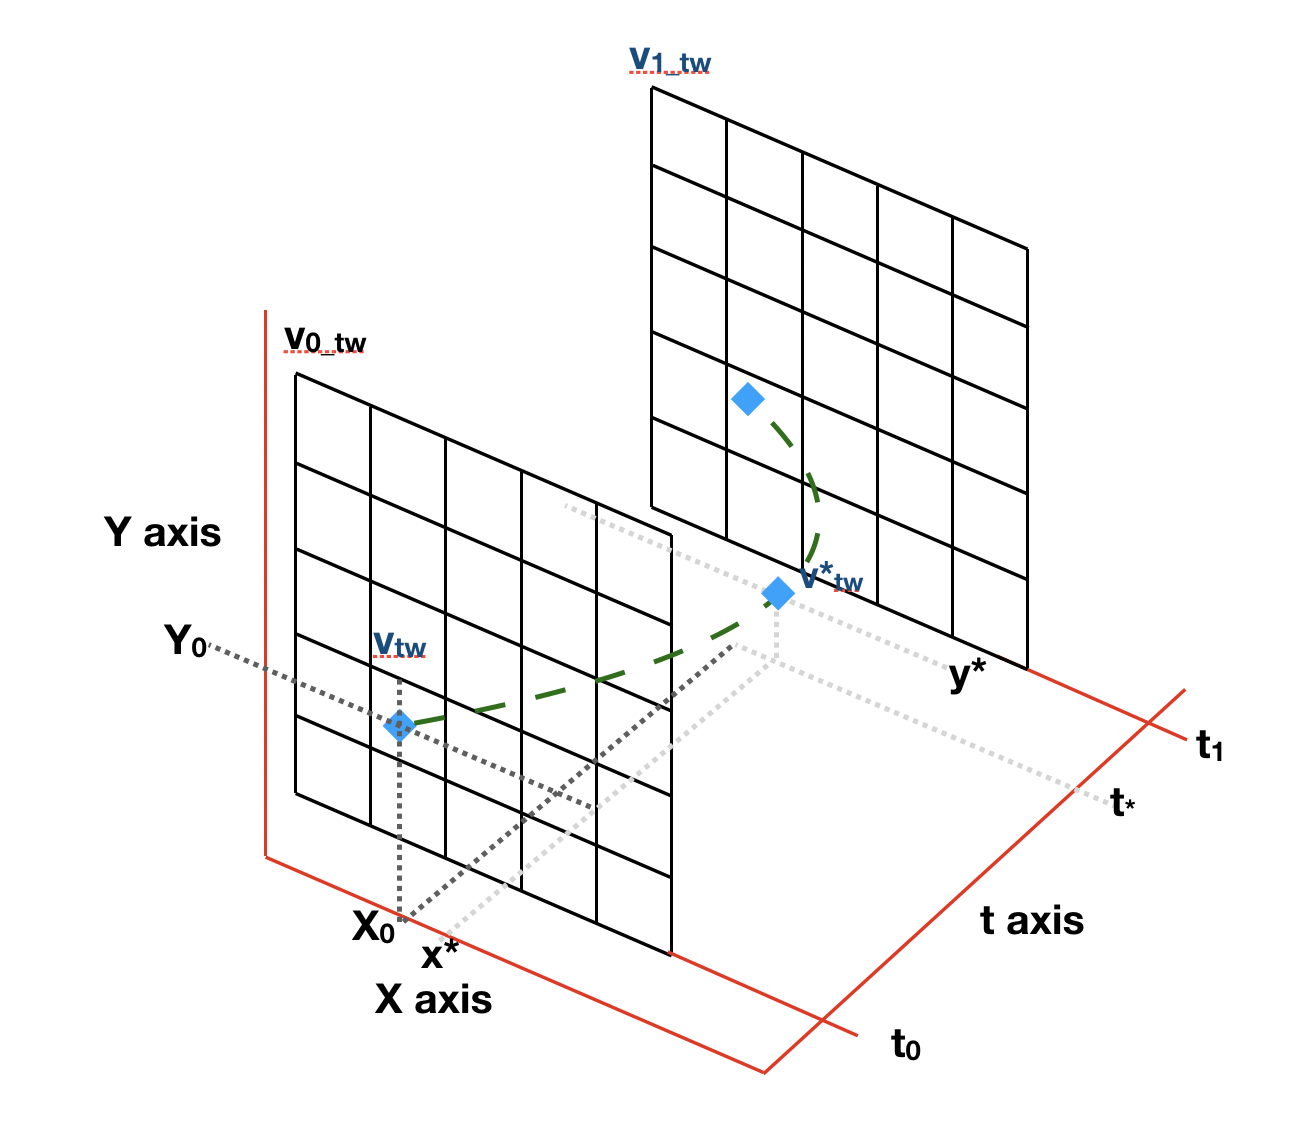
\includegraphics[width=0.45 \linewidth]{gridDataInterp.png}
    \caption{Griddata Method, graphical representation of two datasets. The function interpolates the coordinates and values from the grid to obtain any intermediate value}
    \label{fig:gridDataInterpo}
\end{figure}

The coordinates used along this algorithm are \textit{[X,Y,t]}, this means that any data using \textit{[Lat, Lon]} coordinates have to be converted to \textit{Cartesian coordinates} (\textit{[X,Y]}), such as the buoys coordinates. In the case of the time dimension (\textit{t}), the units of the time step are defined in minutes, and this have to be converted to seconds, moreover the number of digits after the point is only one. \par

The minimal time path algorithm not only requires the characteristics of the boat and athlete to solve the problem, but also constraints. These constraints are related with the state-space variables and they embody the environment within the competition takes place. In addition, to the type of maneuvers commonly used by athletes and sailor to sail from one point to another. But to represent properly the environment the area to sail has to be couple to the wind area so the minimal time path can gets a solution. \par \noindent 
Now that the algorithm has been defined and most of their parameter also, the next section will validate them. At the same, it will be review that the parameters defined such as the number of stages is acceptable. All these to verify that a path developed using this algorithm represent the typical path of the laser class developed during races. \par % to meet the purposes of this research. 
%nm 1852 m
%2nm diamter
\section{Validation of the Algorithm: Results and Considerations}
\label{sec:ValidationAlgo}

The purpose of this section is to verify and validate the functionality of this algorithm to estimate the time of the predicted paths, thus to determine the minimal time path. These paths have to meet the constraints previous established and at the same time evaluate the values for the parameters assigned. Particularly the parameter for the number of stages per leg (\textit{n}) when the wind mode to sail is \textit{upwind}. In addition, to the constant related to the tack loss time ($t_{tack-loss}$) added to each of the shifts on directions of the laser class. By the end of the section the considerations and adjustments on the model required are mentioned in order to solve optimization problem.  \par 

The validation is made on an upwind mode because during this mode the laser class is prone to follow a zig-zag pattern. As a result of this, it was defined that the wind speed (\acrshort{v_tw}) and direction (\acrshort{b_tw}) to be constant over time and space. In the other hand, the number of stages to evaluate begins at one (\textit{(n=1)}), so one shift in direction is made to reach the target.%at least one tack maneuver can be made.
\par 
The setup of the parameters and conditions represent the most simplified conditions to evaluate the algorithm but it can reveal easily if the algorithm works properly or not. The first aspect to review is that the algorithm identify the \textit{no-go-zone}, for this the distance between marks is \textit{0.96 nm} equivalent to 1730 meters and $\Delta \Psi$ is 5\degree. Using these parameters, figure \ref{fig:Onestages_NoGoZone} shows that the algorithm develop more than. 346,000 nodes over the whole area defined inside a rectangle of aprox. 8000$\times 4000 m$; however, many of these points are located above the target's location. The marks on green, only at one side of the start point are the nodes that meet the criteria about the angle and the \textit{no-go-zone}. The other side was not plotted %in this way to avoid confusion 
since the \acrshort{vpp} is assumed symmetrical.\par 

\begin{figure} [hbt!]
    \centering
    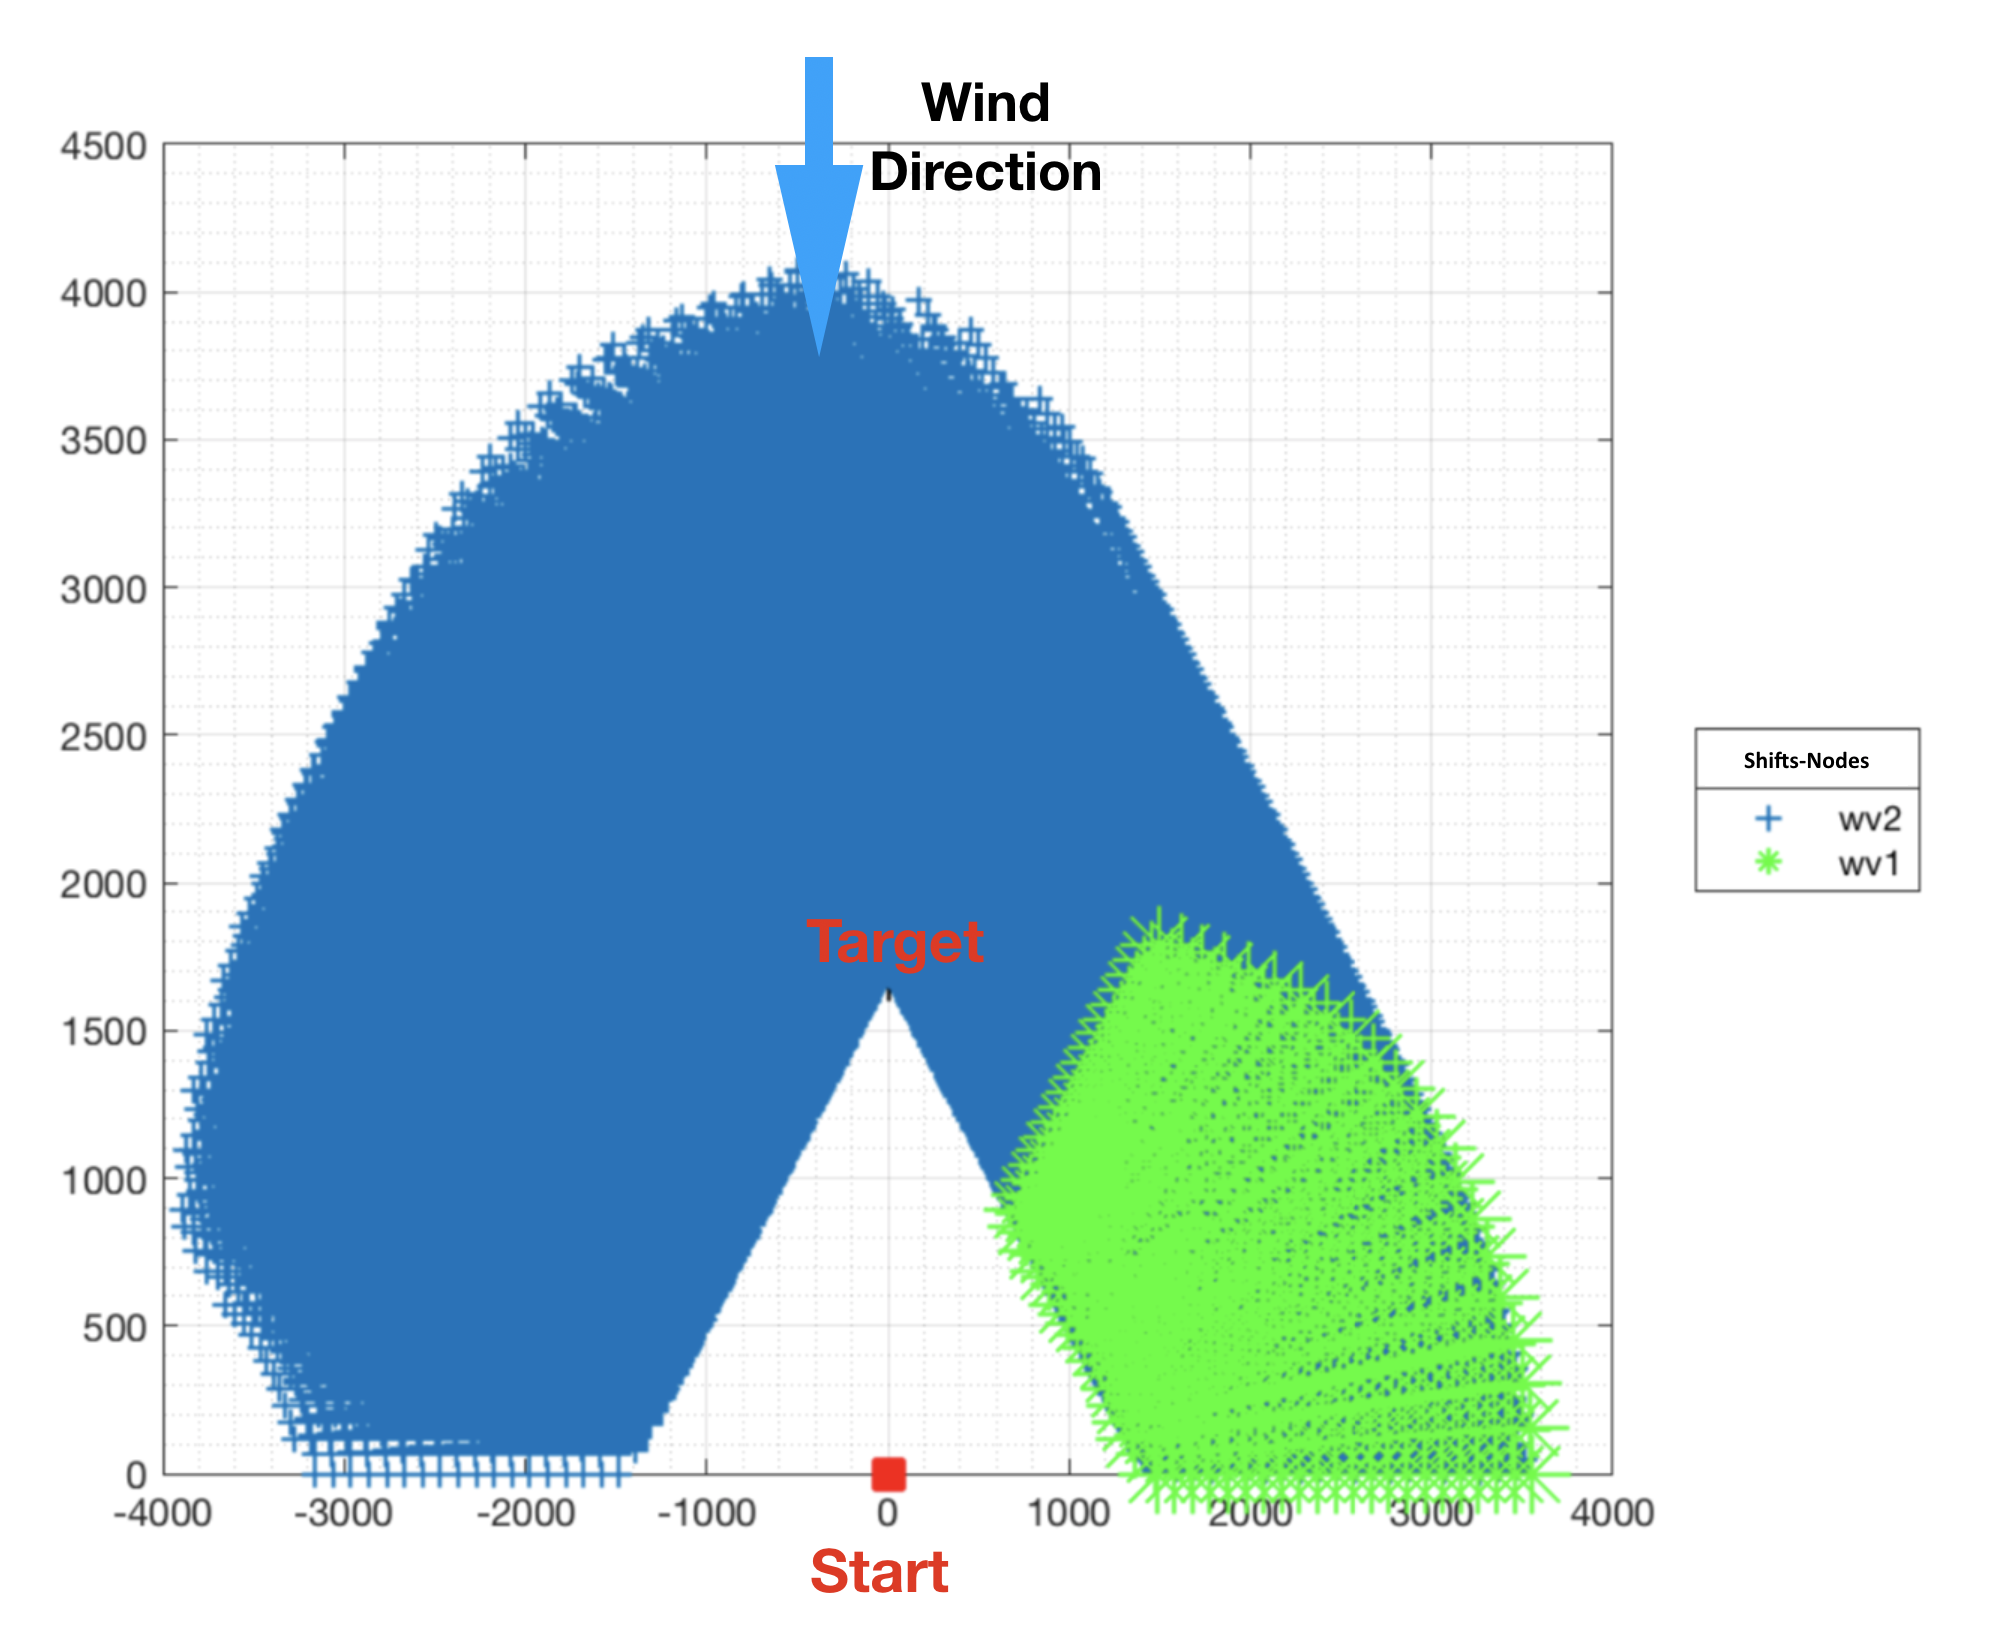
\includegraphics[width=0.45 \linewidth]{images/Nodes_2wv_5deg_5s.png}
    \caption{Nodes generated between 2 marks with one stage \textit{(n=1)} and  $\Delta \Psi = 5 \degree$}
    \label{fig:Onestages_NoGoZone}
\end{figure}

The values for the parameters and conditions to validate the algorithm are shown below. In this case, only half of the angles from the \acrshort{vpp}([0,$\pi$]) was used since it is assumed that it is symmetrical. Moreover, it is assumed constant wind conditions so the paths on both sides from the vertical line on the start mark are symmetrical. These parameter are:
\begin{itemize}
    \item \acrshort{v_tw}= 8.5 kn equivalent to 4.37 $ m/s $.
    \item \acrshort{b_tw}= 0\degree  from \textit{North}. 
    \item The distance between the start line and the next mark is \textit{0.977 nm} equivalent to 1809 meters. %\textit{0.96 nm} equivalent to 1730 meters. %1852 meters.
    \item The number of points stages is two, \textit{(n=2)}.
    \item The time step ($\Delta t$) is 5 seconds.
    \item The heading step angle ($\Delta \Psi$) is 1\degree. %5\degree.
    \item The $t_{tack-loss}$ = 10 seconds.
    \item The tolerance factor for the leg area are for $x_{SAtol}=2.5$ and for $y_{SAtol}=2$.
\end{itemize}

%For the next trial, $\Delta \Psi$ parameter was changed from 5\degree  to 1\degree, and the distance between marks was increased to \textit{0.977 nm} equivalent to 1809 meters, the rest of the parameter remains the same and only one side of the \acrshort{vpp} .
Under these condition more nodes were generated comparing with figure \ref{fig:Onestages_NoGoZone}, and in consequence more paths with even the same time. This is shown on figure \ref{fig:Paths_2wv_1deg_5s} where paths inside the same time range were plotted with the same color. The figure also shows that the fastest paths do not shift after 1200 meter from start point. In fact, figure \ref{fig:PathsTops_2wv_1deg_5s} shows that the paths with the top 5 times shifts before an horizontal distance of 1000 meters, which is only 10.5\% more than the mid-point distance between the marks. Despite the number of paths and its times the target mark hasn't reach perfectly 
%In this case with a smaller $\Delta \Psi$ and a larger distance between marks the paths never reach the target,
this is shown in figure \ref{fig:PathsZoom_2wv_1deg_5s}, where the second best time is the closets path within a radius of 6 meters from the target mark. % and it is the second best time that has this condition. \par
\begin{figure} [hbt!]
  \centering
  \subfloat[Paths generated with \textit{n=1} and $\Delta \Psi =1\degree$.] {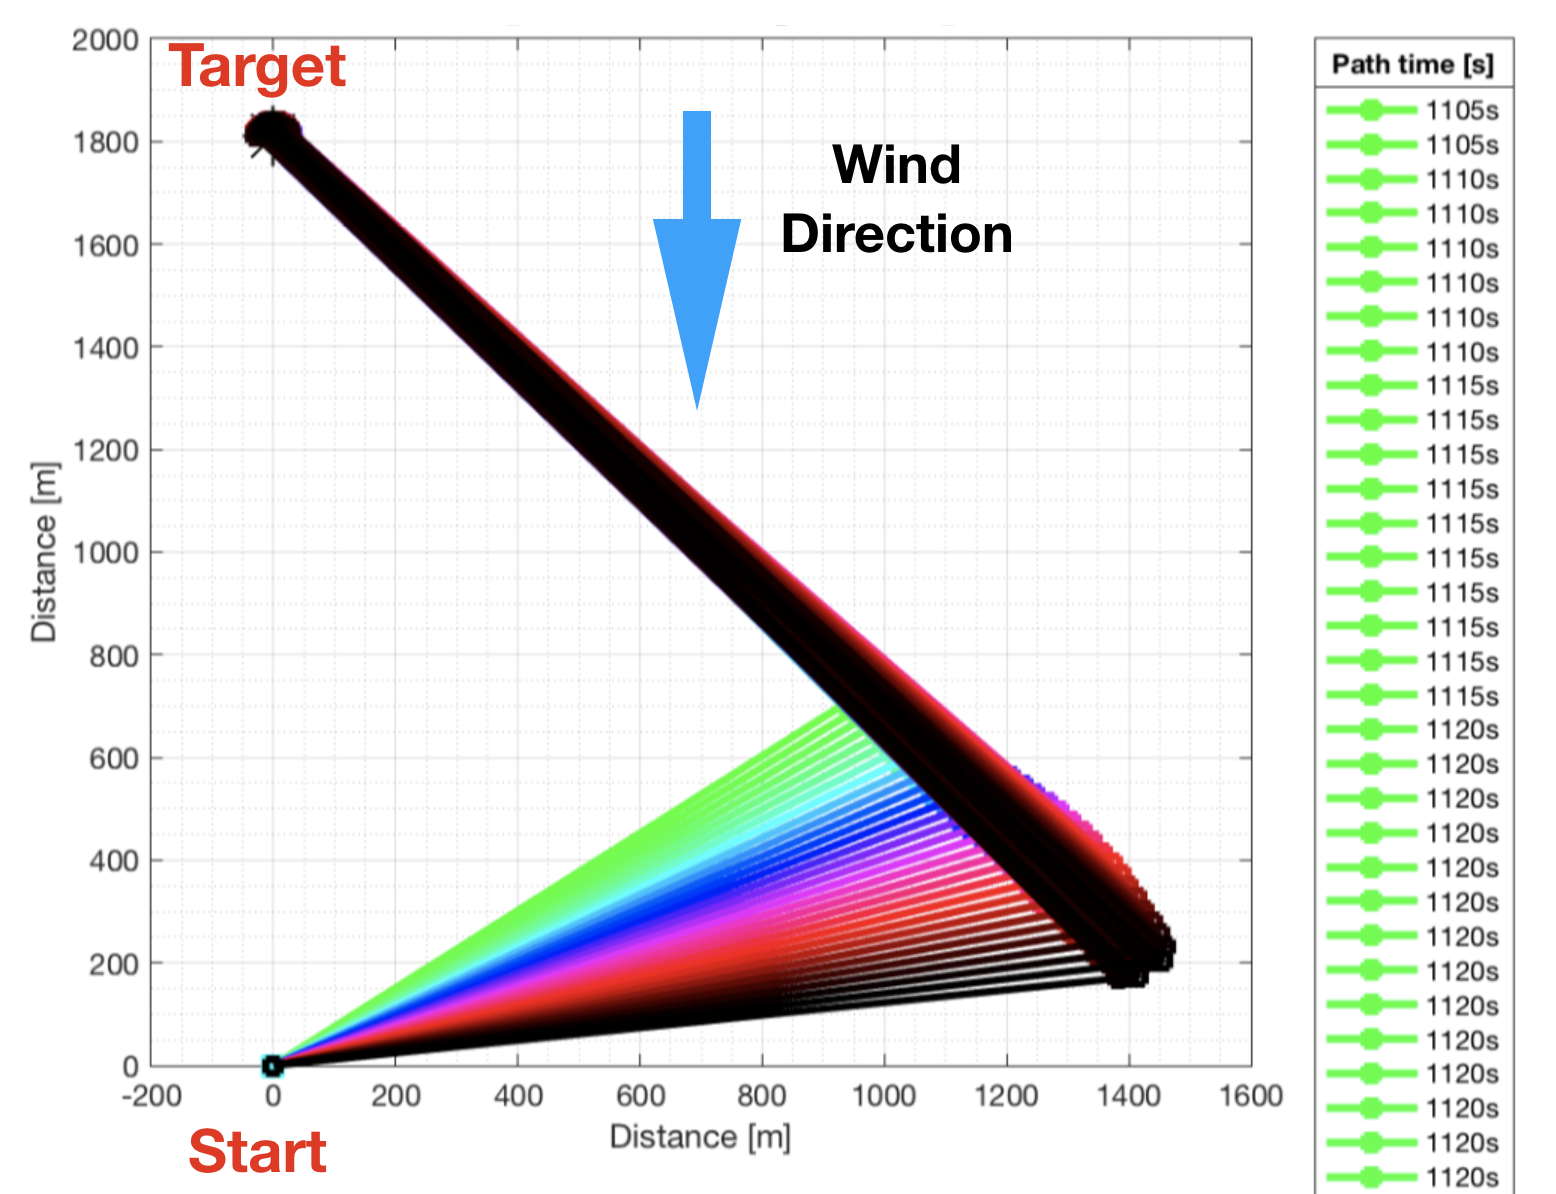
\includegraphics[width=0.31 \linewidth] {images/Paths_2wv_1deg_5s.png} \label{fig:Paths_2wv_1deg_5s}}
  \hfill
  \subfloat[Top 5 time paths and closets to the marked. These paths have the same time.] {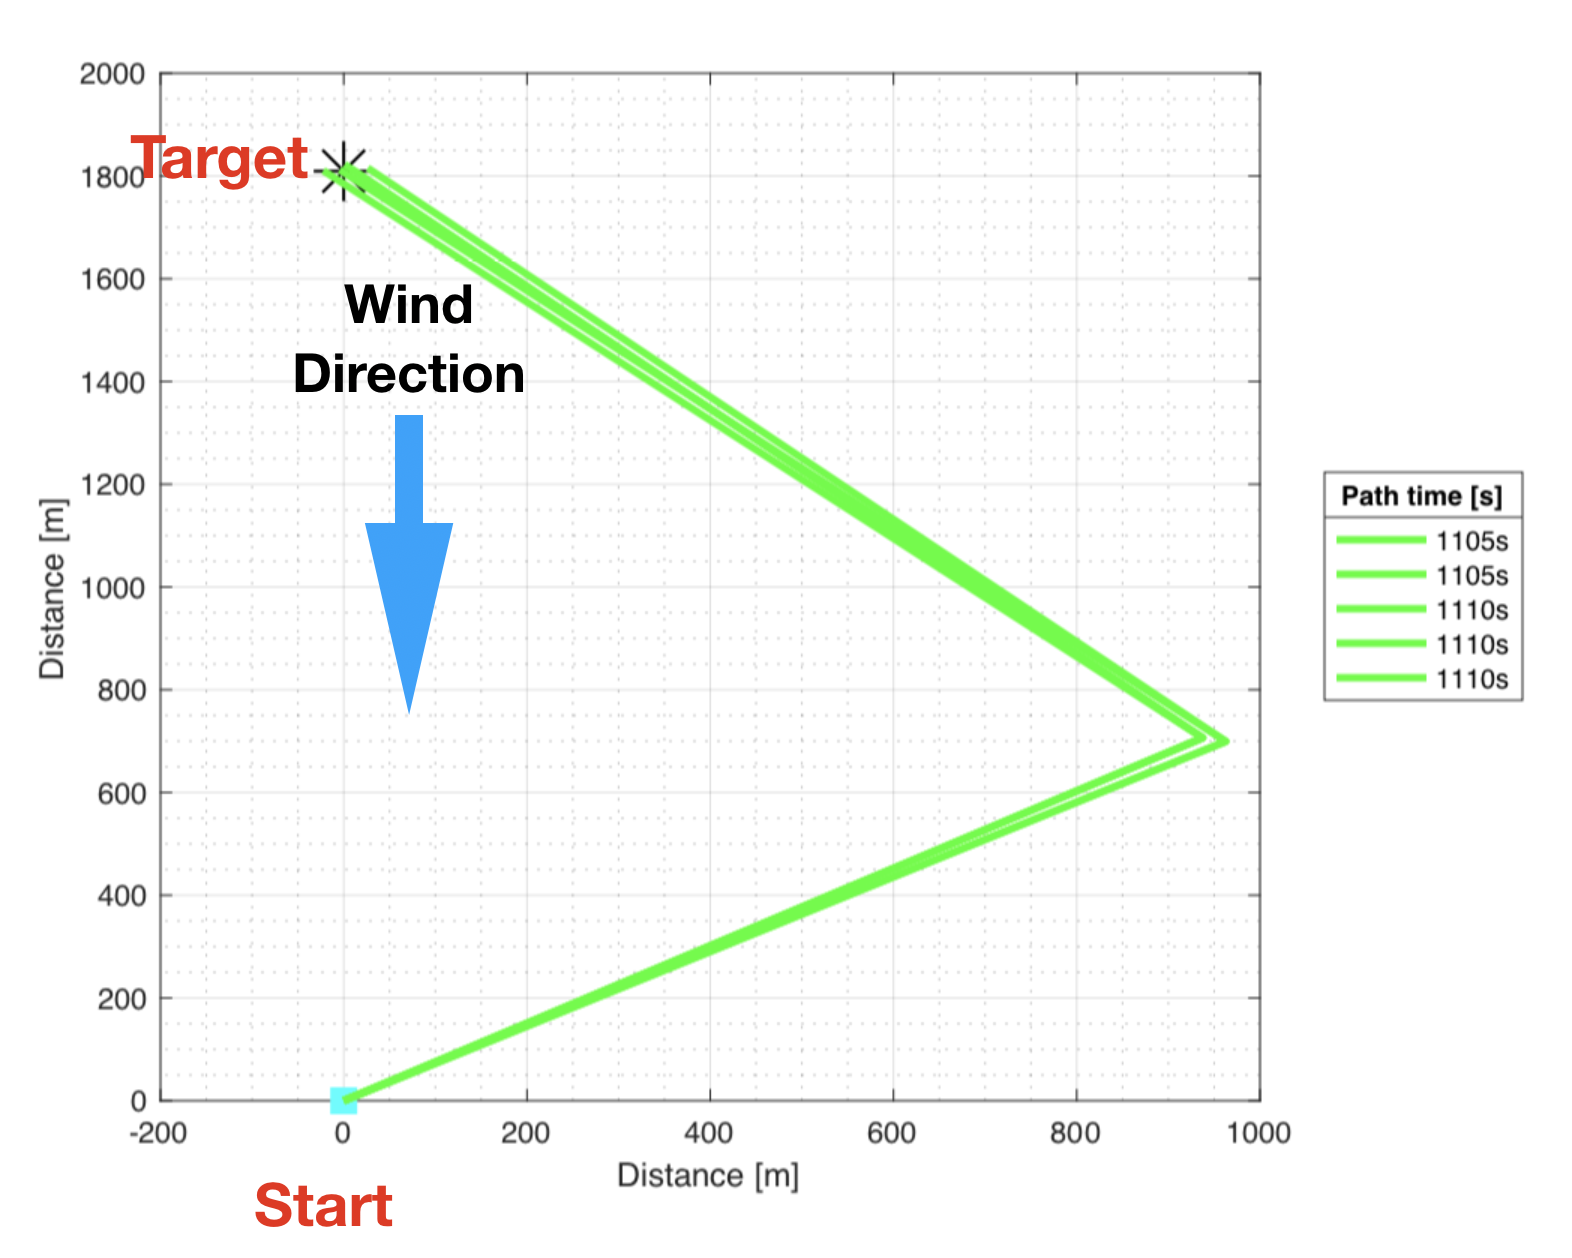
\includegraphics[width=0.31\linewidth]{images/PathsTop_2wv_1deg_5s.png}\label{fig:PathsTops_2wv_1deg_5s}}
  \hfill 
  \subfloat[Minimal time paths close-in end at the target mark.] {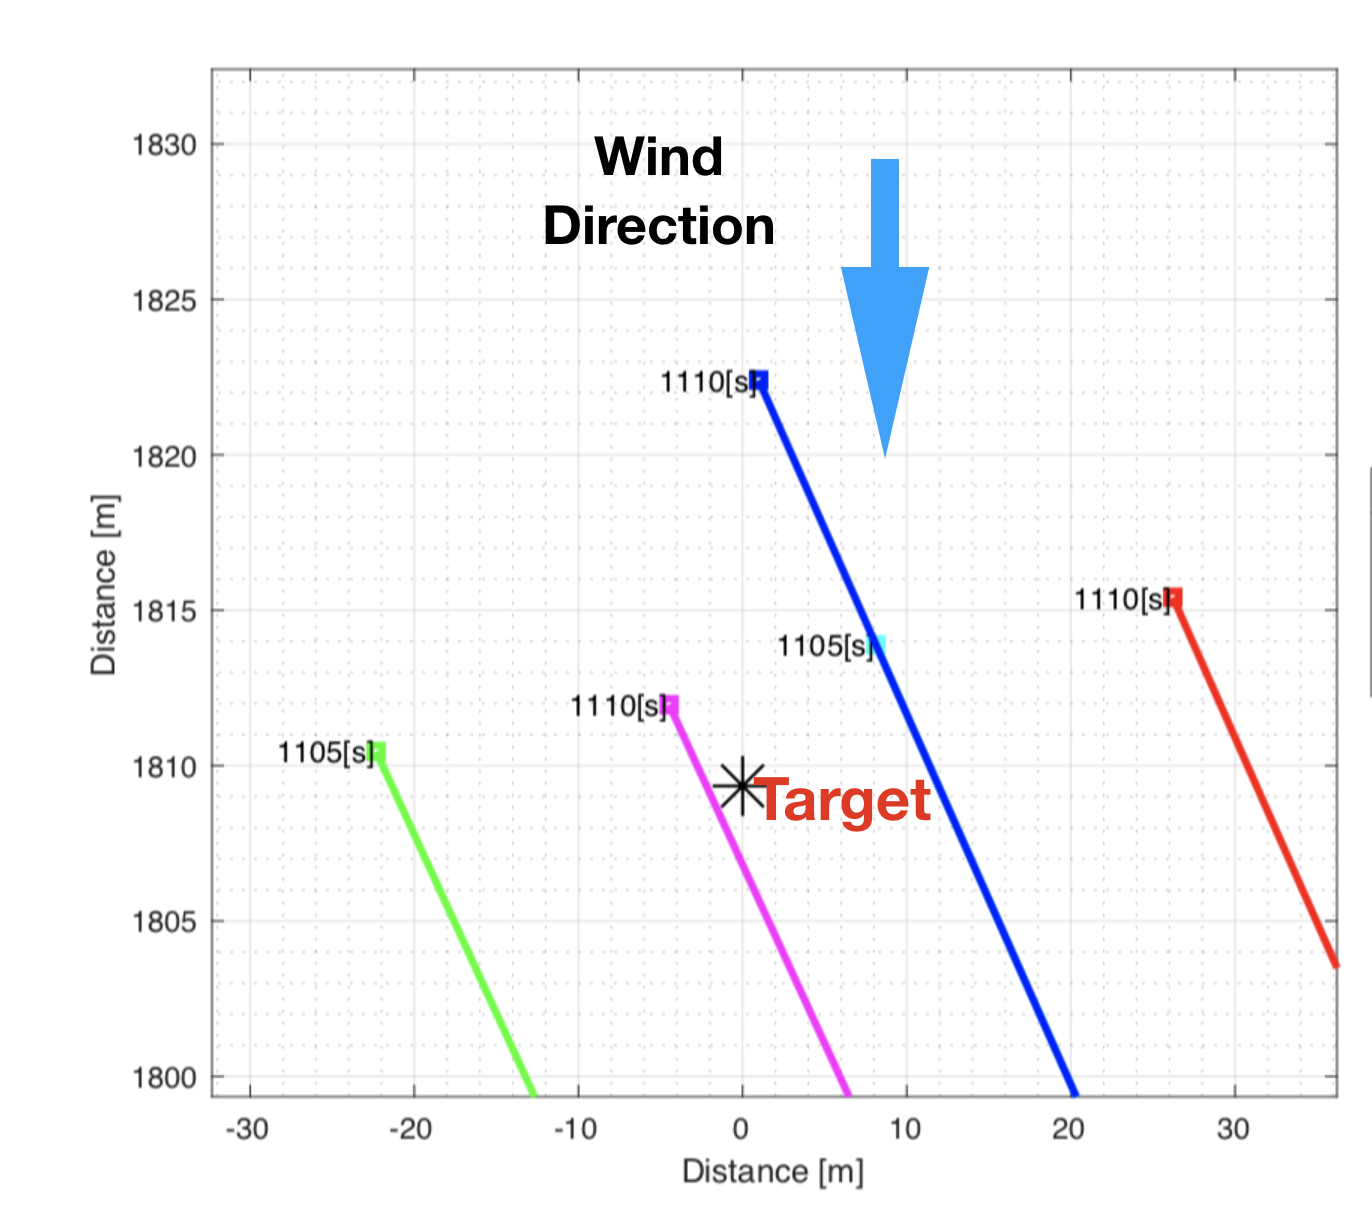
\includegraphics[width=0.31\linewidth] {images/ZoomPaths_2wv_1deg_5s.png} \label{fig:PathsZoom_2wv_1deg_5s}}
  \caption{Paths generated with one shift point in direction (\textit{n=1}) and $\Delta \Psi =1\degree$.}
\label{fig:Nodes_Paths_2wv_1deg_5s}
\end{figure}

When the number of point-stages increase to two (\textit{n=2}), not only the number of nodes and paths increase but the top 5 times also increase by 5 seconds. In this case the first shift in direction occurs at an horizontal distance form the start mark of 1100 meters and following the same heading-angle, figure \ref{fig:Path_3wv_1deg_5s}. The second shift on direction occurs within a radius of 46 meters from the target mark as show in figure \ref{fig:PathZoom_3wv_1deg_5s}. But despite all these alternatives the end of each of the paths does not reach perfectly the target mark. Figure \ref{fig:PathTops_3wv_1deg_5s} shows that all the paths with the same time ends within a radius of 3 meter from the target mark.  \par 

\begin{figure} [hbt!]
  \centering
  \subfloat[Top 5 times using 2 attacks with $\Delta t$ =5s and $\Delta \Psi =1\degree$. All paths have the same time of 1100s] {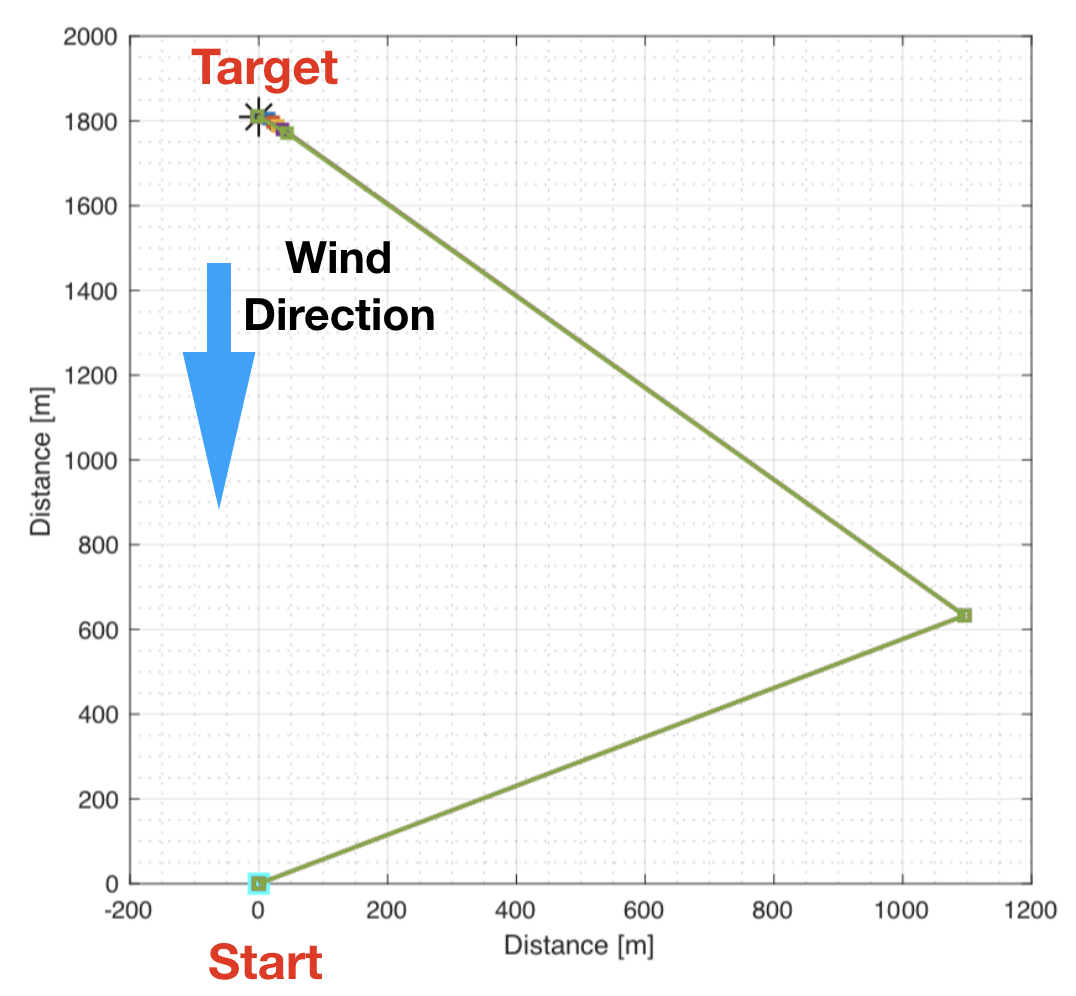
\includegraphics[width=0.31 \linewidth]{images/Paths_3wv_1deg_5s.png} \label{fig:Path_3wv_1deg_5s}}
  \hfill
  \subfloat[Close-up of the top 5 times at the target mark. The ends of paths are within a radius of 3m from the target mark.] {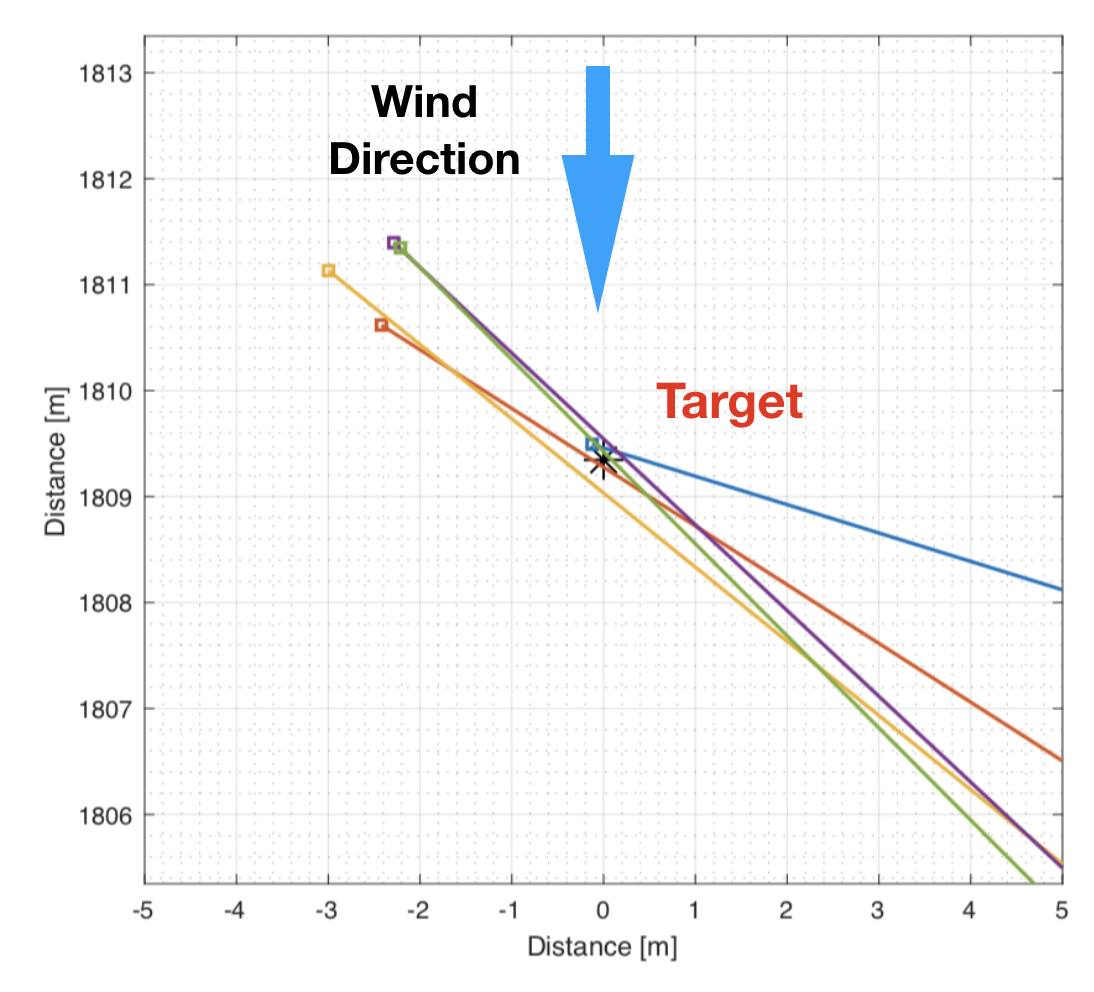
\includegraphics[width=0.31\linewidth]{images/PathsZoom_3wv_1deg_5s.png}\label{fig:PathTops_3wv_1deg_5s}}
  \hfill 
  \subfloat[Details about the shifts on direction after the first heading-direction was taken.] {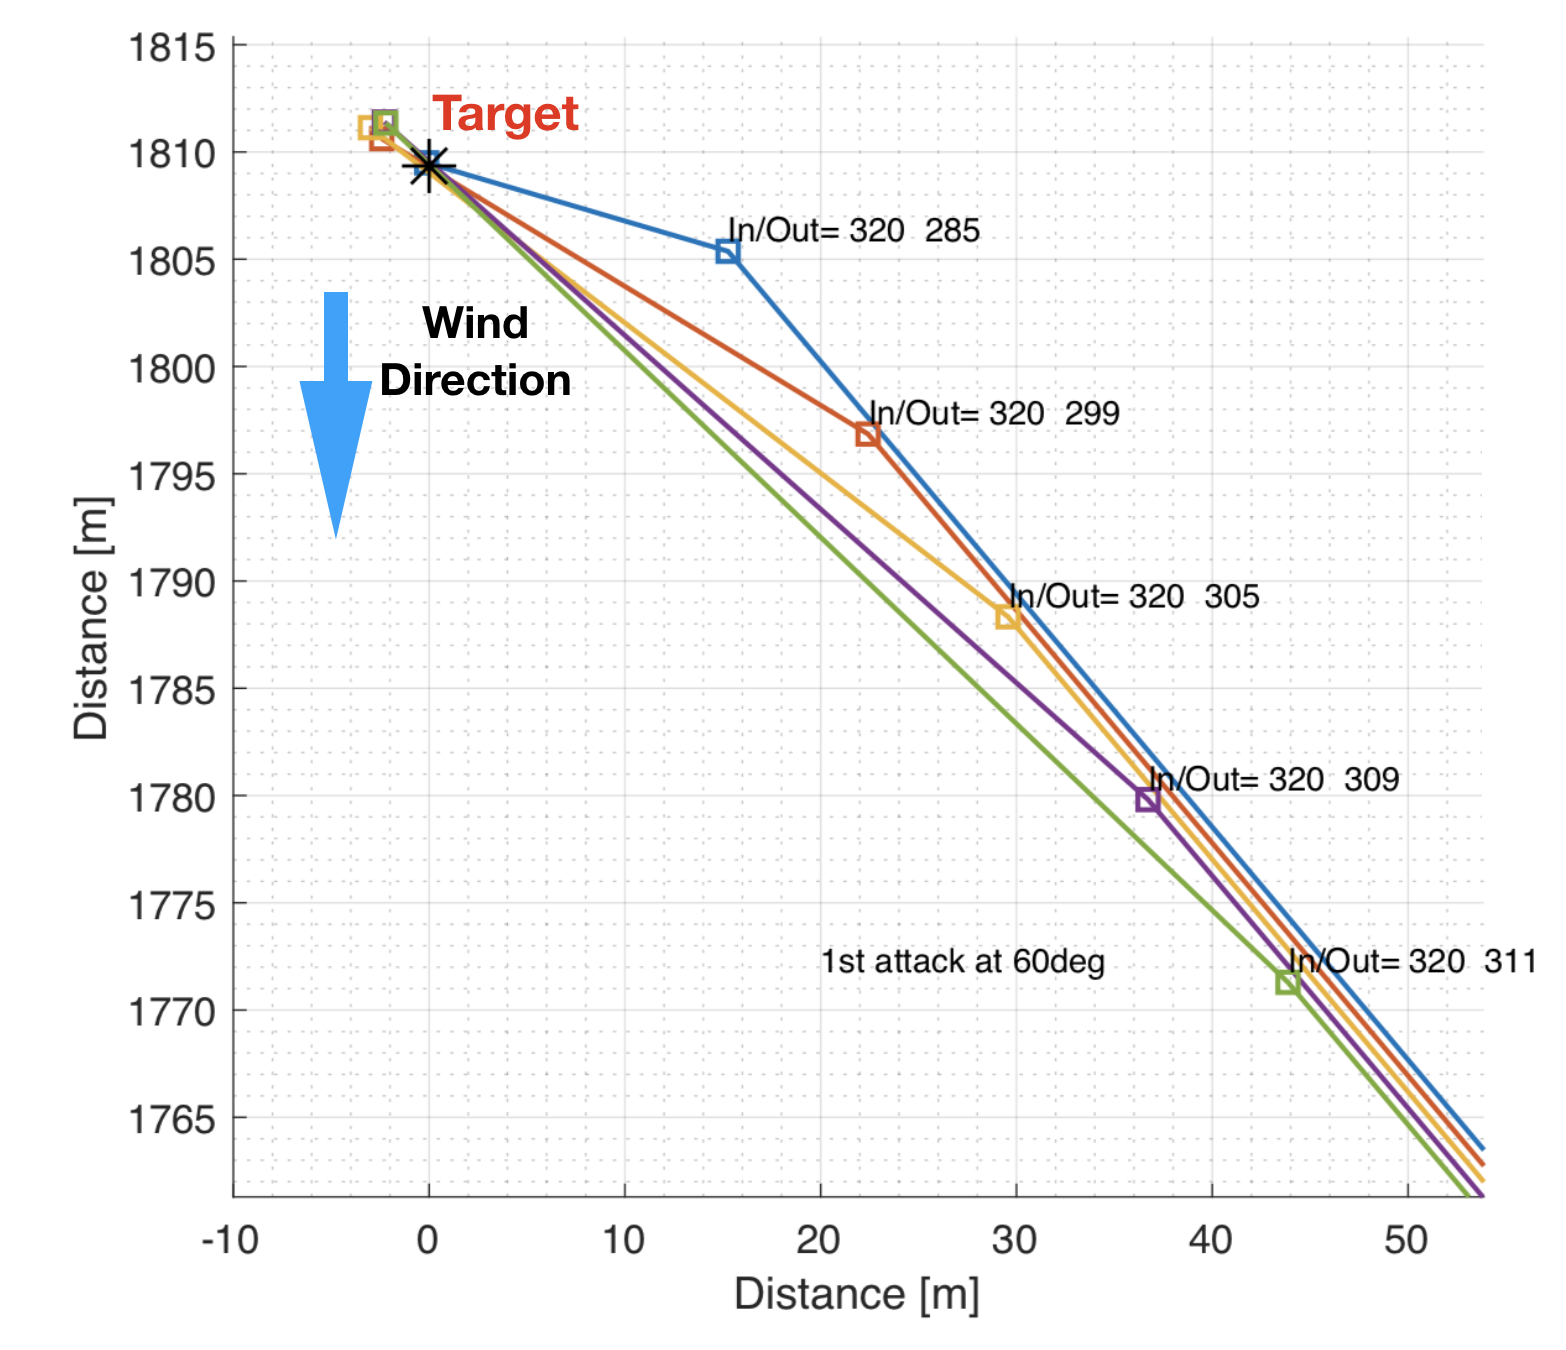
\includegraphics[width=0.31\linewidth] {images/PathsZP_3wv_1deg_5s.png} \label{fig:PathZoom_3wv_1deg_5s}}
  \caption{Top 5 time paths generated with two shift point in direction (\textit{n=2}) and $\Delta \Psi =1\degree$, the time of all them is 1100 seconds.}
  %Top 5 time paths and close-up at the target zone with two shifts in direction with $\Delta \Psi =1\degree$, } %$\Delta t$ =5s and
\label{fig:Paths_3wv_1deg_5s}
\end{figure}

From the previous results, it was clear that either another constrain or other type of adjustments to the algorithm are required to eliminates this kind of solutions. One of this changes refers to the definition of \textit{n}, which is the number of points inside each leg in order to define the number of internal stages within it. To represent this \textit{n} is a point with coordinates \textit{[X,Y]} inside a vector where its first set of values represent the coordinates of the star buoy and the last element are the coordinates of the end buoy. This means that \textit{n} are the number of points inside a vector and regardless the coordinates of these points they are linked to the legs using the buoys. It can be said that \textit{n} defines the size of a vector for the stage-state variables as in equation \ref{eq:n_vector}. \par
\begin{equation} \label{eq:n_vector}
\textrm{stage-state vector} = 
    \begin{bmatrix}
        x_{bouy,start} & y_{bouy,start} \\ 
        x_{1} & y_{1} \\
        \vdots & \vdots\\
        x_{n} & y_{n} \\
        x_{bouy,end} & y_{bouy,end} 
    \end{bmatrix}
\end{equation}

The value of \textit{n} stage points in this research is assigned to be \textit{7}, this means that inside each leg there are 8 stages where a shift in direction could occurs. Besides, at least 70 seconds could be added to the time's path if these shifts occurs along each leg. The locations of these \textit{n} is determined by the space constraints assigned to each leg and by the angle constraints, in other words by equations \ref{eq:Xmin_SailArea} to \ref{eq:Ymax_SailArea}. \par 

\begin{figure}[hbt!]
    \centering
    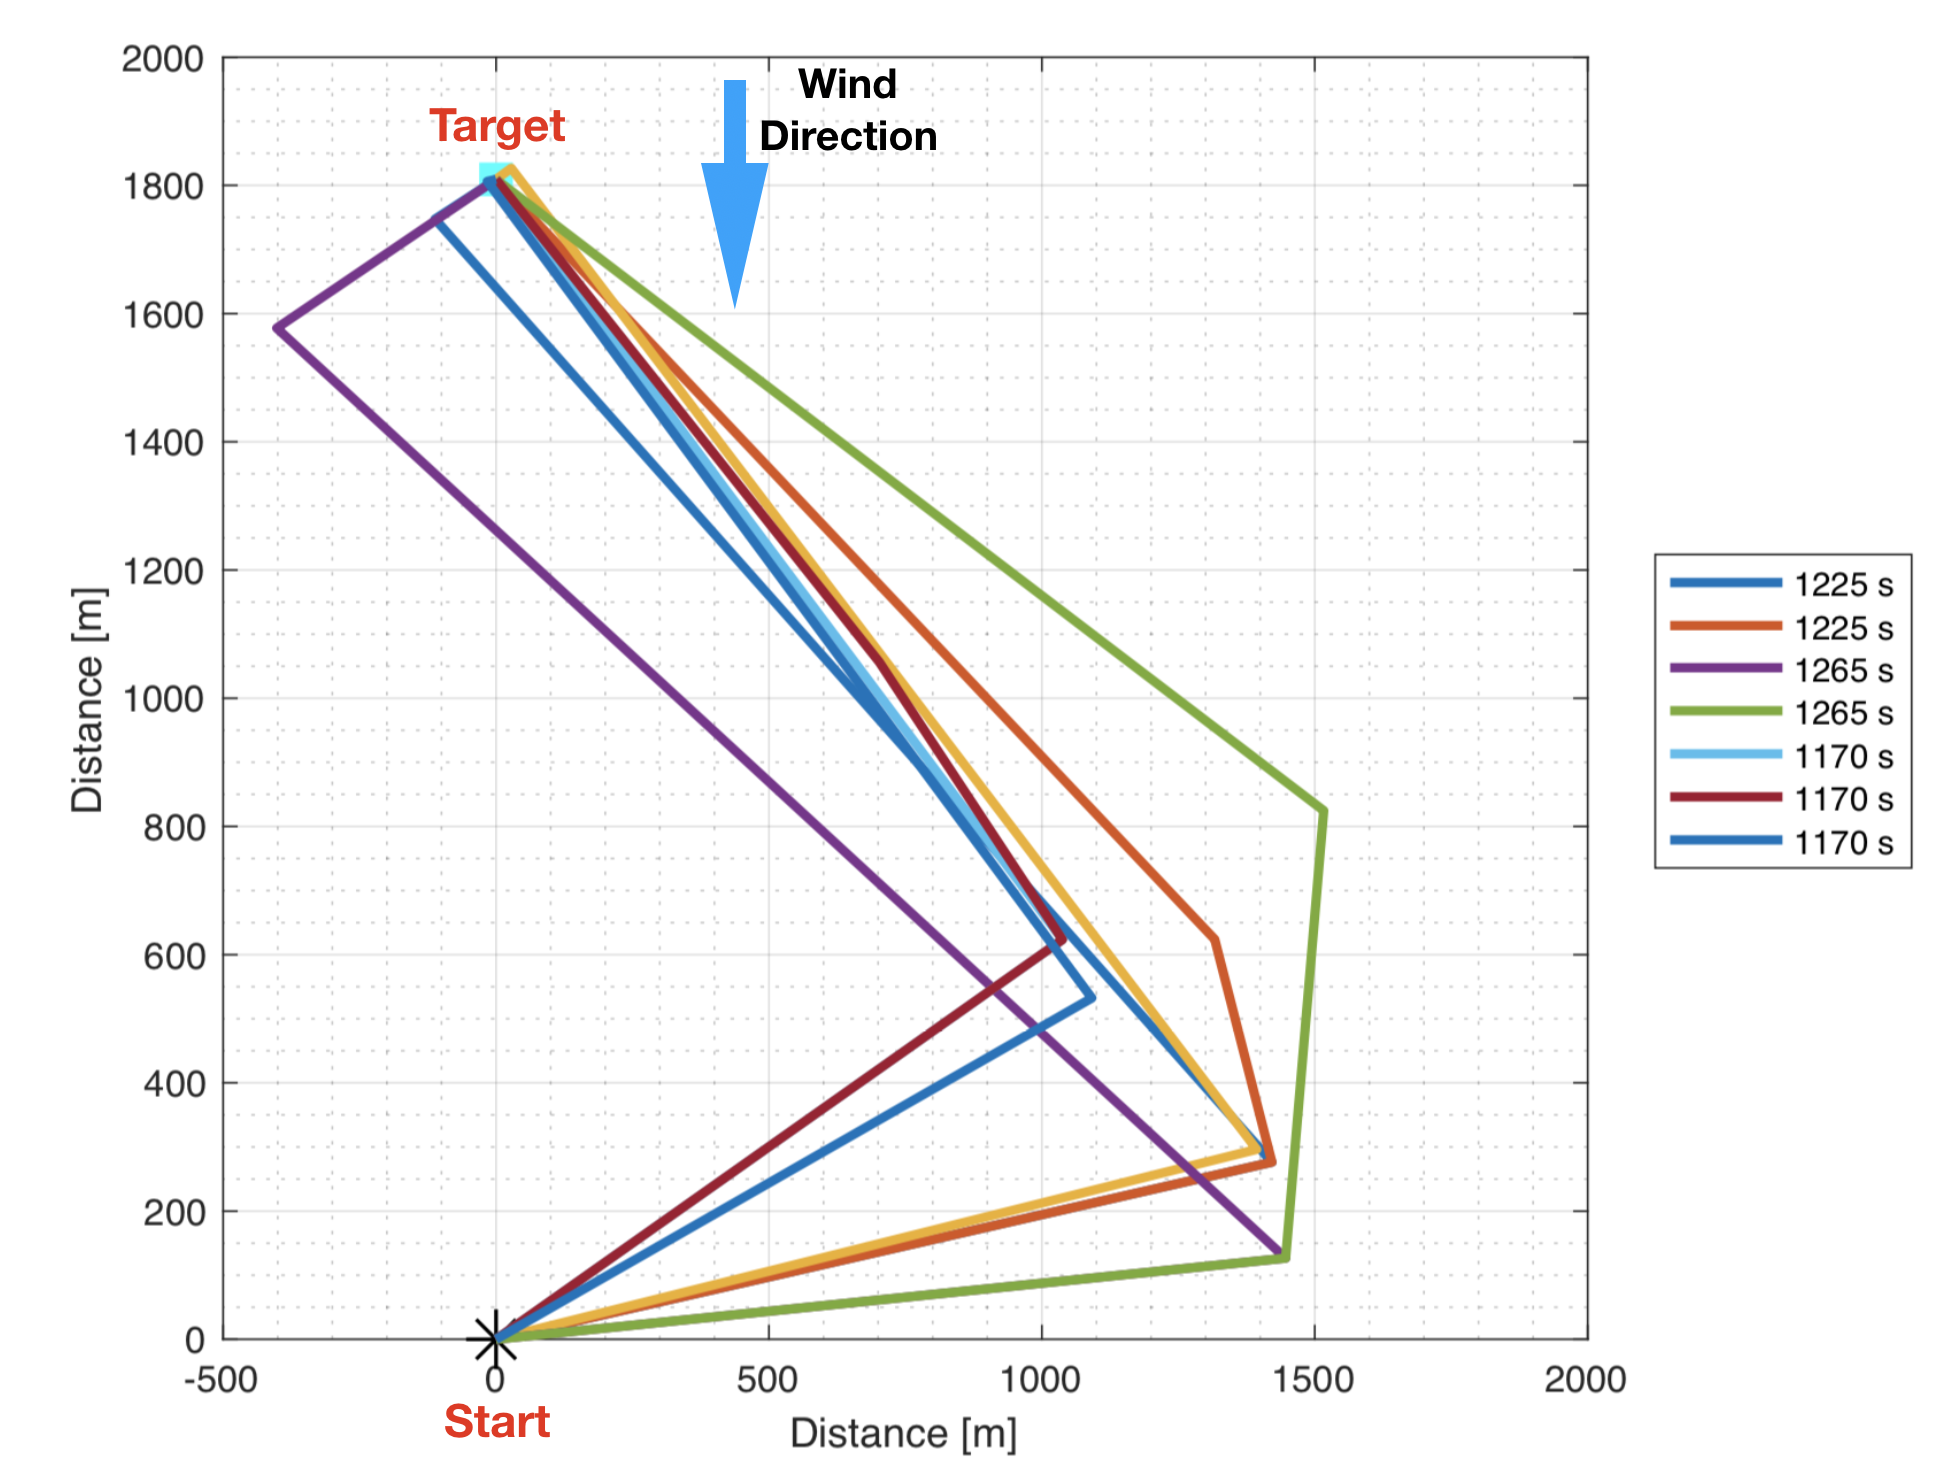
\includegraphics[width=0.45 \linewidth]{sections/n_stage_state_v.png}
    \caption{Paths generated using the stage-state vector \textit{n=2} and $\Delta \Psi =1\degree$}
    \label{fig:n_stage_state_vector_paths}
\end{figure}
Applying this changes figure \ref{fig:n_stage_state_vector_paths} shows some of the paths developed with them. It also shows that the fastest paths make the first shift before 1050 meters at an horizontal distance from the start mark. Furthermore, this distance is 1.15 times the mid-point distance between marks and this ratio is the same when \textit{n=2}, and equations equations \ref{eq:Xmin_SailArea} to \ref{eq:Ymax_SailArea}, use a factor ($x_{SAtol}$ and  $y_{SAtol}$) to scale up the area for each leg. Using these trials  %the maximum coordinate between the two buoys is required. 
equation \ref{eq:SailAreaTol} indicates the value of these tolerance factors, for now it is assumed that the value for each factor is the same for both coordinates. \par

\begin{equation} \label{eq:SailAreaTol}
    x_{SAtol}=y_{SAtol}=1.15
\end{equation}

Applying all thee changes the algorithm can developed paths that meet the constraints and estimate its time. For the optimization problem, particularly for the \textit{fmincon} function, where the option for the internal algorithm has to set as \textit{'active-set'}. This option allows the algorithm to take large steps far from the target so the number of iterations and evaluations of the algorithm are used effectively to find the optimal solution. It was observed that without this change, the solution takes a larger number of iterations and evaluations of the function to get the optimal solution. Besides, most of the time this solution is not even the optimal compared with the solutions provided with the \textit{'active-set'} method. \par 

After making these changes in the algorithm and adding trapezoidal route as figure \ref{fig:Rio_Course1}, with the same \acrshort{v_tw} as previously defining but with \acrshort{b_tw} about 140\degree. The optimal path for the race is shown in figure \ref{fig:Val_route}, where each leg is indicated by a different color, the total time is about 56 minutes. Because the wind is constant in time and space the fastest trajectory in a downwind and direct wind is by following a straight line. \par \noindent 
The optimal path for the upwind mode on leg 1 was found by developing 2 routes where the start conditions meet the constraints.  These two conditions where optimized using the algorithm and the minimal time between them provides the optimal path for the leg. Figure \ref{fig:Val_leg1} shows these 4 paths, the path marked in green was used to construct the optimal path for the race and it was used as a constraint for the second leg. \par 

\begin{figure} [hbt!]
  \centering
  \subfloat[Leg 1, Upwind Mode ] {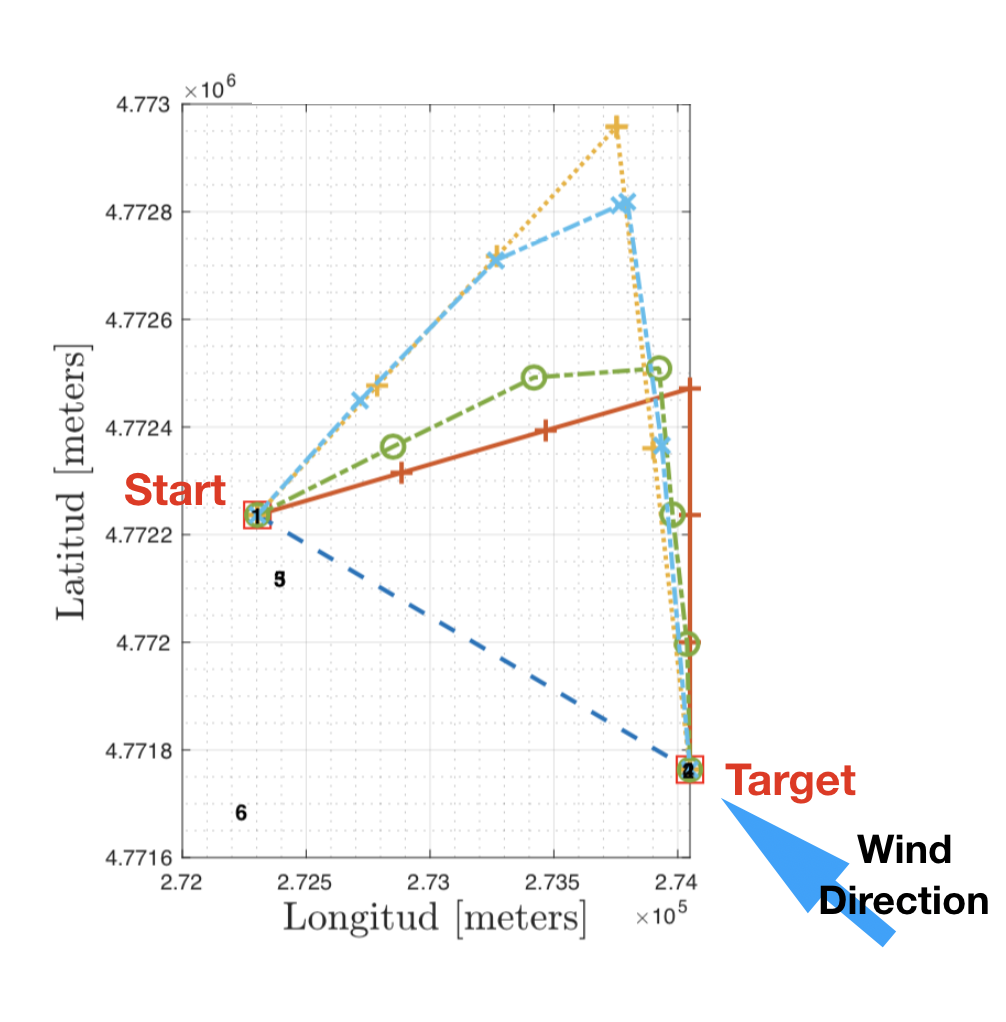
\includegraphics[width=0.4 \linewidth]{sections/Val_leg1.png} \label{fig:Val_leg1}}
  \hfill
  \subfloat[Race Optimal Path per leg] {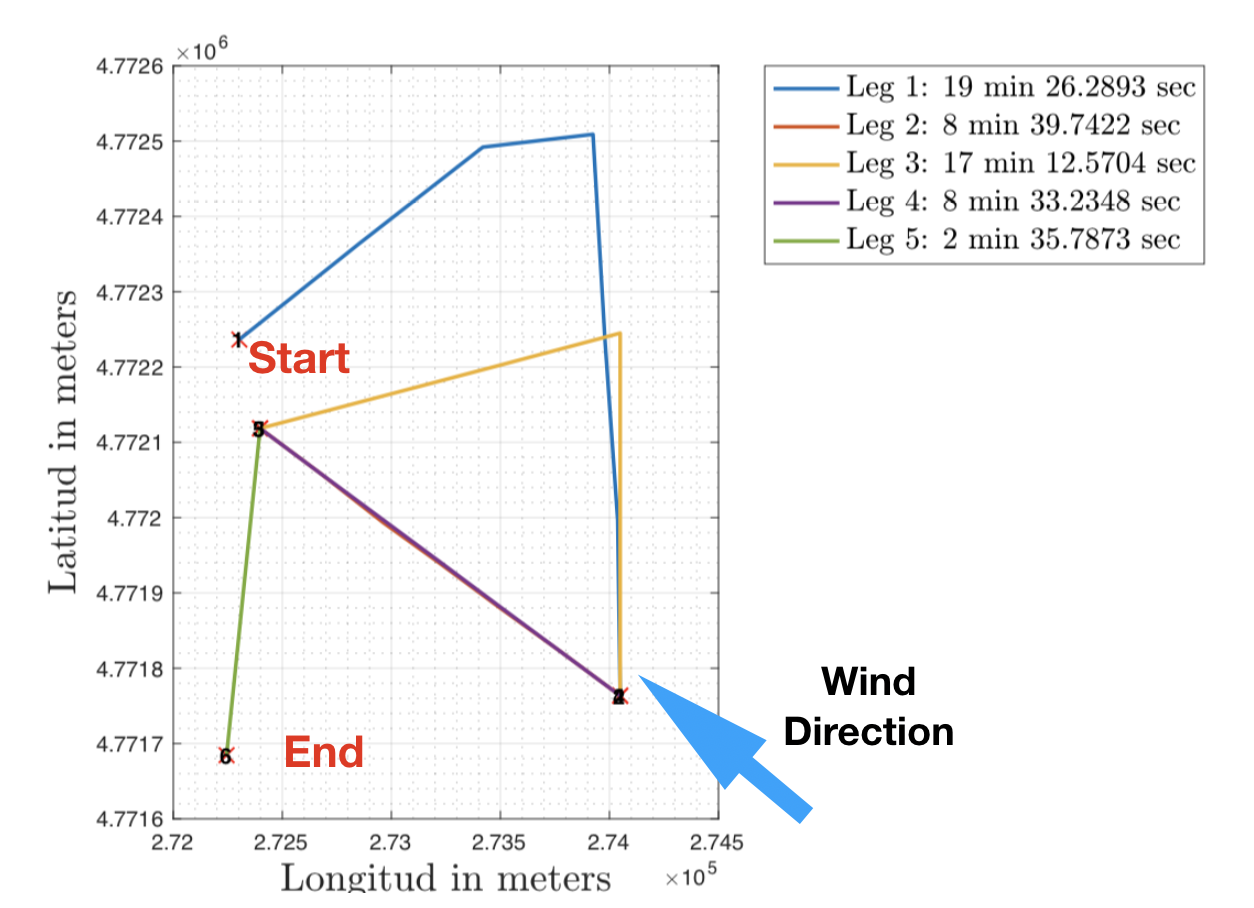
\includegraphics[width=0.525\linewidth]{sections/Val_route.png} \label{fig:Val_route}}

  \caption{Validation} %$\Delta t$ =5s and
\label{fig:Val_algorithm_Route}
\end{figure}

The optimal time path or the minimal time path can be found by finding the minimal times per leg, the initialization of the algorithm requires initial guess for the variables used. Because the system is non-linear due to the no-convex shape of the \acrshort{vpp} the optimal solution is not unique. The algorithm developed considers two initial guess values for the variables, after the optimization is done the results are compared to find the minimal time path between them.  
The algorithm uses the heading-direction approach to find the optimal path, and it divides each leg on stages. \par 
\noindent
These points also controls and limits the number of shifts in direction that define the zig-zag pattern specifically in the upwind mode. % These shifts are particularly common on the upwind mode. 
Furthermore, the points-stages \textit{(n)} inside the leg enable the continuity between legs, this continuity is constrained by the angle between legs and between these points. The locations of these points are limit by the area assigned to each leg, since the space area determine the number of nodes or coordinates where these points can be located. Most important, the area must be contained inside wind model area and it has to be large enough to estimate the wind's velocity (\acrshort{v_tw}) and direction (\acrshort{b_tw}) at any time and location. 
%since a tight area limits the number of datasets available to estimate the wind's velocity (\acrshort{v_tw}) and direction (\acrshort{b_tw}) at any time and location. 
\par Now that the algorithm was validated to developed paths, estimate its time and optimized them to get the minimal time path the next chapter will evaluate 2 conditions for the time-step. 





%at 0\degree (\acrshort{b_tw})  while the distance between the start line and the next buoy is \textit{1 nm} equivalent to 1852 meters and with different valuetimes for the stages. The first condition to test is with only one stage (\textit{n=1}), 


%First to review if the algorithm can make attacks when the wind mode to sail is \textit{upwind} and if the es
%\section{Considerations: Results from  the Validation}
%During the \textit{upwind} wind mode the sailboat is prone to follow a zig-zag pattern 
%Because of this, the wind properties are setup

%[x,y] = mfwdtran(lat,lon)
%\subsection{Wind Model}
%Weather model forecast are calculated  by super computer and updated every three hour according regions. Different agencies have developed models to predict it in global terms. The local prediction are made based on it with via extrapolation and interpolation between local measurements with the intention to predict it every hour, for local purposes. The global and open information is stored in what is know as GRIB or NET files. This files, GRIB, is downloaded according the region of interest the common grid size provides is a 3 km square. 
%In \cite{binns2002development} the simulator use a guts wind model  with the next parameters: the time step was defined as 60 seconds and the length of 200 m. It can be said that the grid 

%definition of the wind area and its implementation into the sail course 

%\begin{figure} [hbt!]
 %   \centering
  %  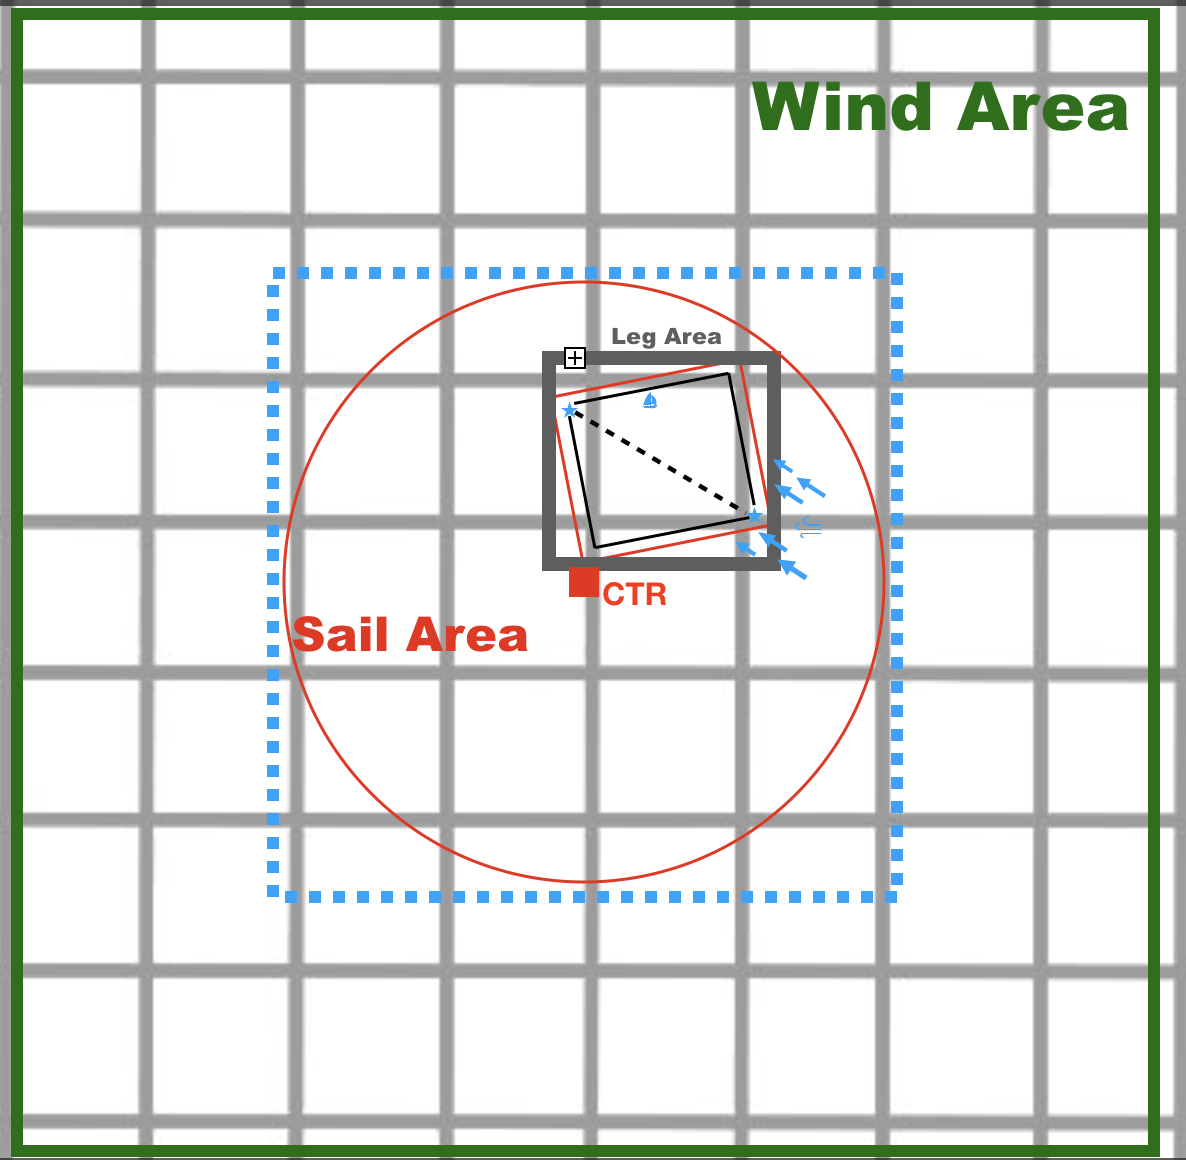
\includegraphics[width=0.5 \linewidth ]{windArea.png}
  %  \caption{Wind Area Concept using a wind model representation. The lines in red are the ctr and limits of the sail area, which can be inscribed on a square.}
   % \label{fig:WindAreaSketchLEG}
%\end{figure}